\documentclass[a4paper, 11pt]{report}
\usepackage[utf8]{inputenc}
\usepackage[T1]{fontenc}
\usepackage{lmodern}
\usepackage{fancyhdr}
\usepackage{epstopdf}
\usepackage{graphicx}
\usepackage{caption}
\usepackage{hyperref}
\usepackage{url}
\usepackage{eurosym}
\usepackage{titlepic}
\usepackage[french]{babel}
\usepackage[top=2cm, right=2cm, bottom=2cm, left=2cm]{geometry}
\usepackage{graphicx}
\usepackage[T1]{fontenc}


\title{REX Minotaure}


\date{2019}

\titlepic{
\includegraphics[width=0.4\textwidth]{images/LogoMinotaure.png}}

\begin{document}

\maketitle

\tableofcontents

\part{Introduction}

Ce REX a pour rôle d'accumuler les connaissances de générations en générations. Souvent, la coupe de france de robotique demandera l'utilisation d'outils spéciaux comme des ventouses mais celles-ci ne seront pas utilisées les années suivantes et les connaissances dessus seront ainsi perdues.

Dès que vous rencontrez quelque chose qui n'est pas dans ce REX, que vous voulez faire part d'une expérience enrichissante, d'une astuce ou d'un problème récurrent, il ne faut hésiter à l'ajouter à ce REX (Objectif: il faut que ce REX soit plus épais que le poly de MMC).

Minotaure ne pourra s'améliorer que si on accumule l'expérience au fur et à mesure des années (chose difficile avec les césures).

\section{Histoire}
Minotaure existe depuis 2004. C'est un P03 qui a créé l'association pour pouvoir continuer à participer à la coupe de france de robotique hors de la mécatronique (il a d'ailleurs créé sa propre entrerprise qui sponsorise des équipes de la coupe de france de robotique).

\section{Rôle de Minotaure}
Minotaure est une association officielle, au même titre que le BDE ou le TRIUM. Son objectif est de permettre aux étudiants de pratiquer la robotique aux Mines. En pratique, cela passe par gérer le budget du cours de Mécatro. En échange, l'association est financée par l'école pour participer à la coupe de France de Robotique.


\section{Les différentes équipes au cours du temps}

\subsection{2015-2016}
\begin{description}
\item[Président:] Matthieu Vignes
\item[Trésorier:] 
\item[Secrétaire générale:]
\end{description}

\subsection{2016-2017}
\begin{description}
\item[Président:] Louis Dattin
\item[Trésorier:] Yoënn Burban
\item[Secrétaire générale:] 
\end{description}

\subsection{2017-2018}
\begin{description}
\item[Président:] Maxence Leroy
\item[Trésorier:] Ulysse Réglade
\item[Secrétaire générale:] 
\end{description}

\subsection{2018-2019}
\begin{description}
\item[Président:] Thomas Gossard
\item[Trésorier:] Léo Chabert
\item[Secrétaire générale:] Louise Fayole
\end{description}

\subsection{2019-2020}
\begin{description}
\item[Président:] Corentin Lemoine
\item[Trésorier:] Adrien Pauron
\item[Secrétaire générale:]
\end{description}

\part{Composants}

\chapter{L'électronique de base}

\section{Les commandements}
\begin{itemize}
\item \textbf{Toujours les composants électroniques seront branchés afin d'avoir une masse commune}
Sinon, les cartes pourront cramés en raison d'une différence de potentiel électrique trop grande.
\item \textbf{Le signal à l'oscilloscope, tu observeras}
Si tu communiques des informations à travers des câbles et tu ne sais pas pourquoi, la première chose à faire et d'observer le signal avec un oscilloscope ou un analyseur logique afin de s'assurer qu'il correspond bien à ce que tu veux.
\item \textbf{Les branchements tu vérifieras avant d'alimenter ton circuit}
C'est si facile de faire une erreur et de détruire des composants.
\item \textbf{Par étapes, tu feras}
Il ne faut pas se fixer des objectifs impossibles: il faut reprendre l'exemple de base, le réimplémenter pour vérifier que tout fonctionne à partir de là et ensuite construire par dessus.
\item \textbf{Organisé tu seras}
Pas besoin d'expliquer pourquoi.
\item \textbf{La documentation tu liras}
Combien de temps j'ai perdu en ne comprenant pas pourquoi ça ne fonctionnait pas alors que la solution était dans la documentation.
\item \textbf{Une fois tes soudures terminées, aux multimètres tu les vérifieras}
\end{itemize}

\section{Précautions}
\begin{description}
\item[Manipulation de circuit intégré:] Plus les composants sont petits, moins ils sont résistants. Il faut notamment faire attention avec les circuits intégrés. L'électricité statique peut les endommager. Pour se décharger, il suffit de toucher un objet relier à la terre comme la prise terre d'une prise électrique ou le boîtier métallique d'un ordinateur.
\end{description}

\chapter{Actionneurs}

\section{Moteurs pas-à-pas}

\begin{figure}[h!]
\begin{centering}
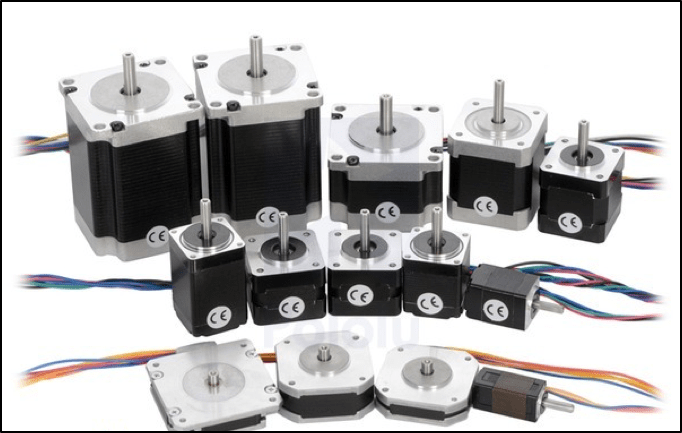
\includegraphics[width=0.4\textwidth]{images/MoteurPasAPas.png}
\caption{Moteur pas-à-pas}
\par\end{centering}
\end{figure}

Les moteurs pas-à-pas sont des moteurs synchrones électriques brushless à courant continu. Il en existe 3 types:
\begin{description}
\item[Moteurs pas-à-pas à aimants permanents] Un aimant permanent est solidaire de l'axe du moteur (rotor). Des bobines excitatrices sont placées sur la paroi du moteur (stator) et sont alimentées chronologiquement. Le rotor s'oriente suivant le champ magnétique créé par les bobines.
\item[Moteurs pas-à-pas à reluctance variable] Il s'agit d'un moteur qui comporte un rotor à encoches se positionnant dans la direction de la plus faible réluctance. Ce rotor, en fer doux, comporte moins de dents qu'il n'y a de pôles au stator.
\item[Moteurs pas-à-pas hybrides synchrones]Ils combinent les 2 technologies précédentes, et sont pluschers. Leur intérêt réside dans un meilleur couple, une vitesse plus élevée. Vidéos explicatives des moteurs pas-à-pas hybrides: \url{https://www.youtube.com/watch?v=eyqwLiowZiU}
\end{description}

\begin{figure}[h!]
\begin{centering}
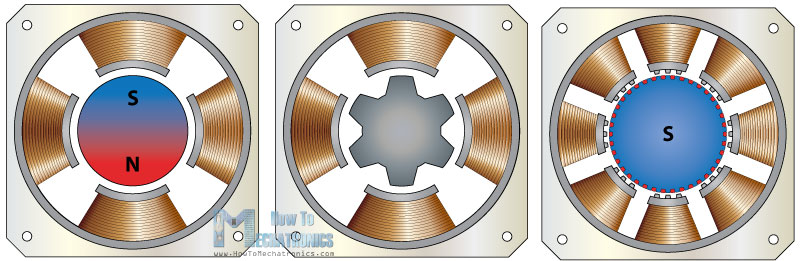
\includegraphics[width=0.4\textwidth]{images/DifferentsMPP.jpg}
\caption{De gauche à droite: Aiment permanent, Reluctance Variable, Hybride}
\par\end{centering}
\end{figure}

Le nombre de phase d'un moteur correspond au nombre de bobines indépendantes. Ce nombre est proportionnel à la précision du moteur.
Parmi les moteurs pas-à-pas à 2 phases, il existe 2 sous-groupes:
\begin{description}
\item[Unipolaire:]Les plus simples d'utilisation et moins chers. Leur connecteur est constitué de 6 fils. Chaque pôle est constituée de deux bobines enroulées en sens inverse sur les pôles du stator. Pour changer le sens du champ magnétique dans un pôle, il faut alimenter l'une ou l'autre de ces deux bobines. Le sens du courant est constant.
\item[Bipolaire:]Les plus puissants. Leur connecteur est constitué de 4 fils. Chaque pôle du stator est constitué d'une seule bobine, et nécessite donc deux fils d'alimentation. Le sens du courant change tout le temps.
\end{description}

Les moteur les plus courants sont ceux à aimants permanents et les hybrides.

\textbf{Utilisation:} Imprimantes (3D ou simple), photocopieurs, robotique, pousse-seringue,...

\textbf{Avantages:}
\begin{itemize}
\item Contrôle en position possible donc en vitesse sans avoir besoin d'une boucle fermée
\item Précision
\item Existence d'un couple d'arrêt
\end{itemize}

\textbf{Inconveinients:}
\begin{itemize}
\item Le couple maximal est inversement proportionnel à la vitesse maximal, c'est-à-dire qu'un moteur pas-à-pas sera capable de fournir le plus de couple pour de faible vitesse de rotation.
\item Lent, ils ne dépassent pas les 3000 tr/min en général.
\item Volumineux et lourd
\item Fonctionnement plus complexe qu'un moteur à courant continu
\item Résonance du moteur
\end{itemize}

\textbf{Précautions:}
\begin{itemize}
\item Le bobinage des moteurs pas-à-pas est très fragile. Si les cables sont mals branchés, il peut y avoir un court-circuit entre les 2 bobinages ce qui "cassera" le moteur pas-à-pas. Il faut utiliser un ohmmètre pour distinguer les fils. 2 fils reliés à la même bobine auront une résistance tandis que d'autres connections afficheront soit rien soit une très grande résistance.
\item Toujours manipuler les fils quand il n'y a pas de courant. Un court-circuit peut facilement détruire les moteurs.
\end{itemize}

Pour distinguer les différents moteurs pas-à-pas, la norme NEMA est utilisée. Cette norme indique la taille du moteur et donc sa puissance. Le nombre représente la surface de la face de l'axe du moteur en pouce carré. Ainsi, un moteur NEMA 11 aura une face d'une surface de 1,1 pouces carrés.

Le couple du moteur est proportionnel au courant.

Une bonne documentation fournira la vitesse et la puissance d'un moteur pas-à-pas. Cependant, il se peut que cela ne soit pas le cas. Dans ce genre de situation, il est possible de calculer des indicateurs sur la vitesse:

\begin{figure}[h!]
\begin{centering}
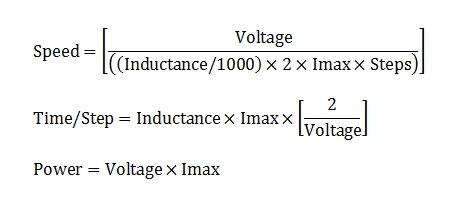
\includegraphics[width=0.4\textwidth]{images/SpeedCalculator.jpeg}
\caption{Calcul de la vitesse d'un moteur pas-à-pas}
\par\end{centering}
\end{figure}

Une version en ligne permet de faire le calcul directement.
\url{https://www.daycounter.com/Calculators/Stepper-Motor-Calculator.phtml}

\textbf{Fournisseurs:} Stepper Online, Gotronic,...

\begin{figure}[h!]
\begin{centering}
\caption{Gauche: Graphique du couple de maintien en fonction du courant consommé - Droite: Réponse en angle à un échelon}
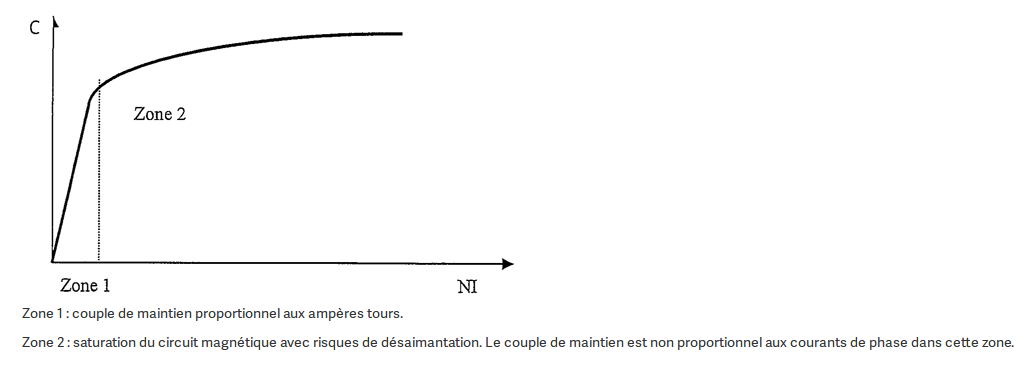
\includegraphics[width=0.4\textwidth]{images/CoupleMaintien.png}
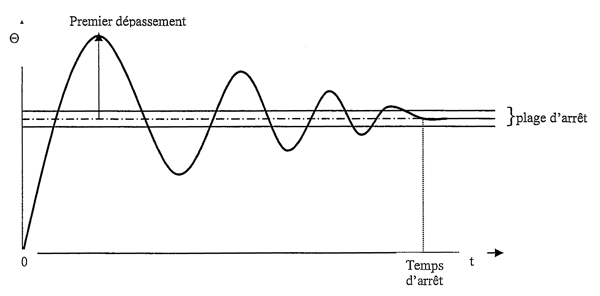
\includegraphics[width=0.4\textwidth]{images/reponse_indicielleMPP.png}
\par\end{centering}
\end{figure}

Pour plus d'information techniques, regarder: \url{https://www.mdp.fr/documentation/lexique/pas-a-pas/notions-techniques.html}

\subsection{Utilisation}

Ce site donne une bonne présentation des moteurs pas-à-pas et comment les utiliser: \url{https://eskimon.fr/tuto-arduino-603-a-petits-pas-le-moteur-pas-\%C3\%A0-pas#se-servir-du-moteur}

Sinon, le contrôleur de moteurs pas-à-pas utlisé pour l'édition 2019 était celui-ci:

\url{https://fr.rs-online.com/web/p/kits-de-developpement-pour-commande-de-moteur/1646982}

Un driver en C a été écrit par Matthieu Vignes et est disponible sur le Git.

\section{Moteurs à courant continu}

Les moteurs à courant continu sont les plus courants. Ils ne sont cependant utilisés que dans des cas basiques.

\begin{figure}[h!]
\begin{centering}
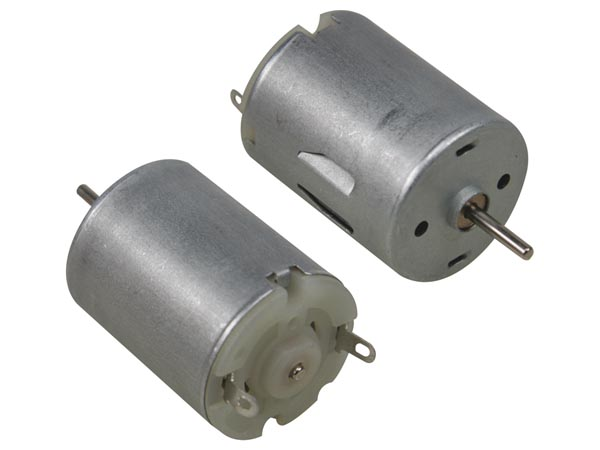
\includegraphics[width=0.4\textwidth]{images/MoteurDC.jpeg}
\caption{Moteurs à courant continu}
\par\end{centering}
\end{figure}

\textbf{Avantages:}
\begin{itemize}
\item Très simple d'utilisation
\item Taille faible pour un couple puissant
\end{itemize}

\textbf{Inconvénients:}
\begin{itemize}
\item La loi entre la tension aux bornes du moteur et la vitesse de rotation ne sera pas la même pour des modèles identiques de moteur.
\item Aucun retour d'information et contrôle en position ou en vitesse impossible en boucle ouverte.
\end{itemize}

\textbf{Fournisseurs:} Conrad, GoTronic, Farnell, ...


\subsection{Utilisation}
Pour un moteur à courant continu, la vitesse de rotation est propotionnelle à la tension à ses bornes. Cependant, étant donné qu'il est difficile de générer une tension variable, le moteur DC est le plus souvent alimenté à travers un hacher avec une tension fixe.

\begin{figure}[h!]
\begin{centering}
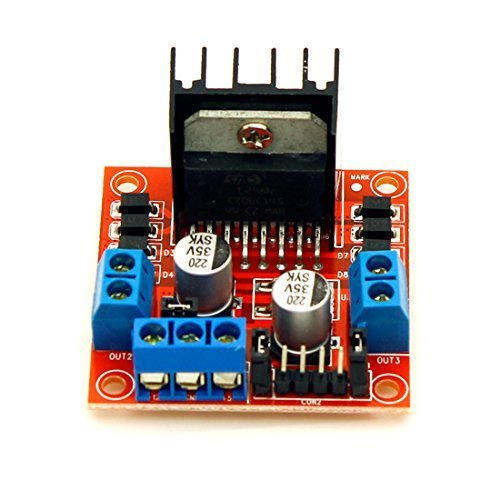
\includegraphics[width=0.4\textwidth]{images/L298N.jpg}
\caption{Pont H L298N}
\par\end{centering}
\end{figure}

Le pont L298N est la meilleure méthode pour contrôler des moteurs à courant continu: \url{https://wiki.mchobby.be/index.php?title=Pont-H_L298N}


Il est aussi possible de de choisir la tension à fournir pour contrôler le moteur avec des transistors:

\url{https://openclassrooms.com/fr/courses/2778161-programmez-vos-premiers-montages-avec-arduino/3285333-le-moteur-a-courant-continu-partie-1-transistors-et-sorties-pwm}

Cependant, le moteur ne pourra tourner que dans un sens avec l'utilisation de transistors.

\section{Moteurs brushless}
Les moteurs brushless comme leur nom l'indique sont des moteurs à courant continu sans balais. De ce fait, ils s'usent moins rapidement que les moteurs. Ils sont  utilisés en aéromodélisme pour leur endurance et la puissance qu'ils peuvent délivrer. A la place des balais, 3 câbles d'alimentations sont nécessaires pour les phases des différentes bobines (alimentation triphasée).

Pour inverser le sens de rotation d'un moteur brushless, il suffit d'inverser la connexion de 2 de ses 3 .

\begin{figure}[h!]
\begin{centering}
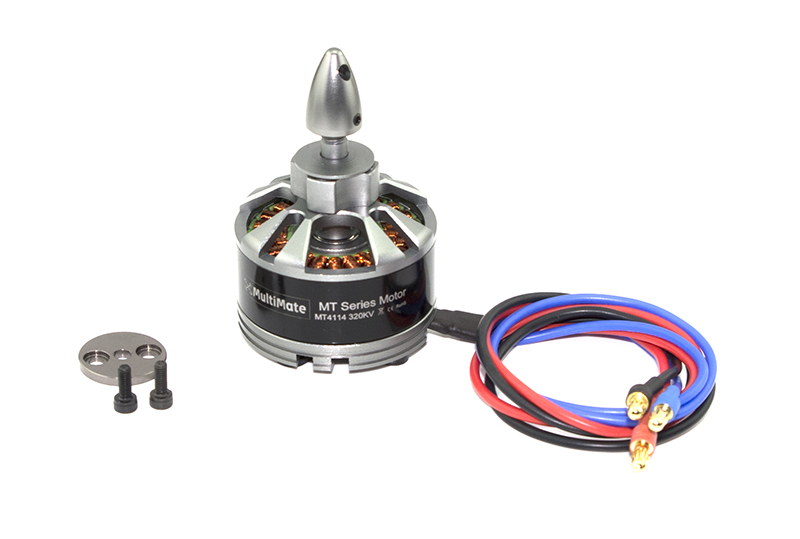
\includegraphics[width=0.4\textwidth]{images/MoteurBrushless.jpg}
\caption{Moteur brushless}
\par\end{centering}
\end{figure}

\textbf{Avantages:}
\begin{itemize}
\item Vitesse asservie
\item Fabriqué pour tourné à de grandes vitesses
\end{itemize}

\textbf{Inconvénients:}
\begin{itemize}
\item Nécessité d'un ESC
\end{itemize}

\textbf{Fournisseurs:} HobbyKing ou autres sites de modélismes

\subsection{Critères de sélection}
\begin{description}
\item[KV:]C'est le rapport tours par minute(RPM)/tension(V). 
\item[Taille:] Un moteur brushless sera décrit par 4 chiffres, 2208 par exemple. C'est sa taille. Les 2 premiers chiffres sont le diamètre et les 2 suivant la hauteur du moteur.
\item[Courant consommé:] L'ESC sera à choisir en conséquence
\item[Batterie:]La notice indique le type de batterie pouvant être utilisé(2S, 3S, ...). Cela revient à indiquer les tensions que le moteur supporte.
\item[Type:]Il existe 2 grands types de moteurs brushless: outrunner et inrunner. Cela indique si le rotor est à l'extérieur ou à l'intérieur.
\item[Le nombre de pôles:]
\end{description}


\subsection{Utilisation}
Pour utiliser un moteur brushless, il est nécessaire d'utiliser un  ESC (Electronic Speed Controller). Un ESC va convertir une tension continu en une alimentation alternative synchrone pour le moteur à travers 3 fils. Ces 3 fils sont interchangeables mais cela changera le sens de rotation du moteur. La tension d'entrée de l'ESC n'est pas unique. Il faut juste qu'elle soit dans l'intervalle demandée. La tension n'aura pas d'influence sur la vitesse de rotation du moteur contrairement au moteur à courant continu. La vitesse de rotation est commandée par un signal PWM en entrée de l'ESC.

Certaines ESC sont équipées de BEC (Battery Eliminator Circuit), c'est à dire qu'il adapte la tension de sortie de la batterie afin de pouvoir fournir une tension utilisable par d'autres éléments électroniques comme un récepteur ou des servomoteurs. En général, un BEC sortira 5V. Voir la section sur les BEC pour plus d'information.

Ce site web explique plus en détail le fonctionnement des moteurs brushless et des ESC:\url{ https://howtomechatronics.com/how-it-works/how-brushless-motor-and-esc-work/}

\begin{figure}[h!]
\begin{centering}
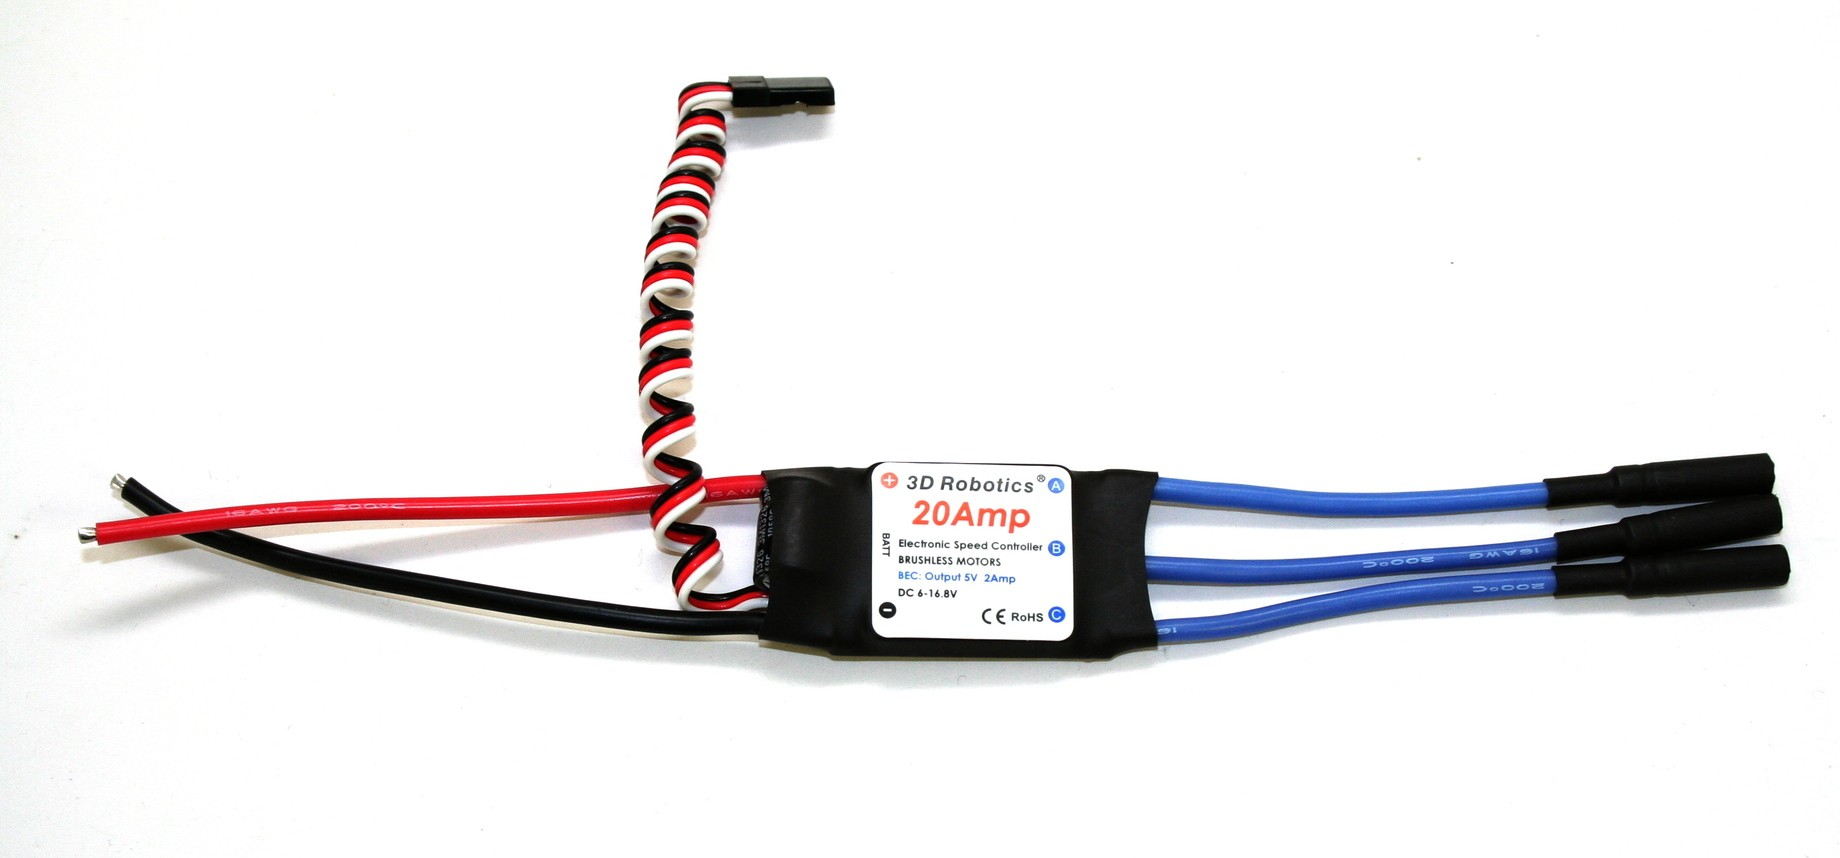
\includegraphics[width=0.4\textwidth]{images/ESC.jpg}
\caption{ESC}
\par\end{centering}
\end{figure}

\section{Servomoteurs}

\begin{figure}[h!]
\begin{centering}
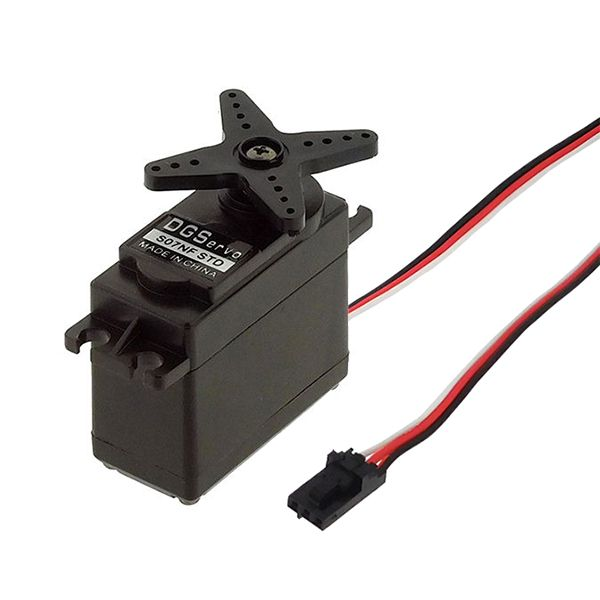
\includegraphics[width=0.4\textwidth]{images/servomoteur.jpg}
\caption{Servomoteurs}
\par\end{centering}
\end{figure}

C'est un moteur à courant continu asservi. Il est souvent utiliser pour effectuer de petits mouvements. On le commande en angle et il maintient ensuite sa position peut importe l'effort exercé dessus (bien sûr il casse si on force trop).



\begin{figure}[h!]
\begin{centering}
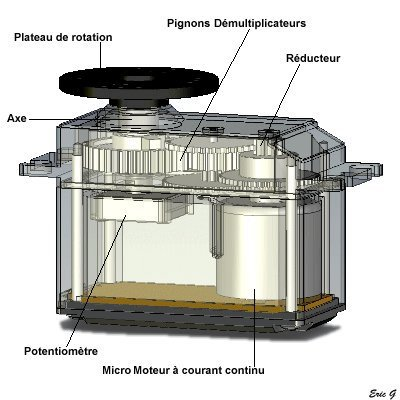
\includegraphics[width=0.5\textwidth]{images/schemaServo.jpg}
\caption{Schéma d'un servomoteur}
\par\end{centering}
\end{figure}

Il est composé d'un moteur à courant continu, d'une réducteur, d'un potentiomètre et d'un circuit intégré. C'est le potentiomètre qui fournit le retour en angle (d'où l'impossibilté de positioner de manière absolue sur plus de 180\degre)

\textbf{Avantages:}
\begin{itemize}
\item Simple d'utilisation
\item Contrôle en position
\end{itemize}

\textbf{Inconveignients:}
\begin{itemize}
\item Aucun retour sur la position
\item Limité à 160-180 \degre de rotation (Il existe cependant des servos à rotation continu)
\end{itemize}

\textbf{Fournisseurs:} Hobbyking (et autres sites de modélisme), Gotronic, Conrad,...

\subsection{Critères de sélections}
\begin{description}
\item[Le couple:]Celui-ci peut être exprimé dans pleins d'unités différentes (N.m, kg.cm, oz.inch, ...). Une fois dans le système d'unité voulu, il suffit de multiplier le couple par le bras de levier (distance entre le centre de rotation et le point d'application de la force).
\item[Taille:]La taille est normalement proportionnelle au couple mais en y mettant le prix, on peut avoir des servos plus petits mais plus puissants.
\item[Tension d'alimentation:]Généralement, les servomoteurs sont alimentés par du 5V. Cependant, pour des plus grands modèles la tension peut passer à 7.4V ou 12V.
\item[Courant:]Le courant consommé par le servo est proportionnel au couple demandé comme pour un moteur à courant continu normal. Il faut prévoir l'alimentation en conséquence. Si jamais il y a un pic de consommation, une chute de tension peut survenir dans tout le circuit ce qui peut provoquer l'arrêt de la carte électronique contrôlant le robot.
\end{description}


\subsection{Utilisation}

\subsubsection{Cablage}

\begin{figure}[h!]
\begin{centering}
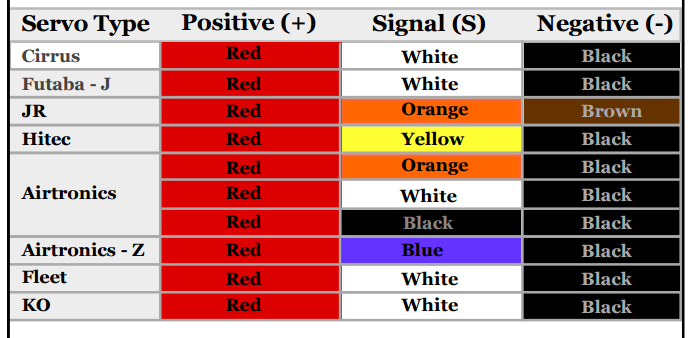
\includegraphics[width=0.5\textwidth]{images/colorCodeCableServo.png}
\caption{Cablage d'un servomoteur}
\par\end{centering}
\end{figure}

Il faut 3 cables pour utiliser un servomoteur:
\begin{itemize}
\item Masse
\item V+ : cela dépend des servomoteirs mais ce sera en général 5V
\item Signal: un signal PWM est utilisé pour commander 
\end{itemize}

\section{Les Dynamixels}
Ce sont les actionneurs le plus souvent utilisés en robotique. Ils sont produits exclusivement par la société Robotis.

En général, ce sont les AX-12 qui sont utilisés. Attention, il faut distinguer 2 modèles d'AX-12: AX-12W qui ont une plus grande vitesse de rotation mais un plus faible couple et les AX-12A qui sont ont un couple plus grand.

\begin{figure}[h!]
\begin{centering}
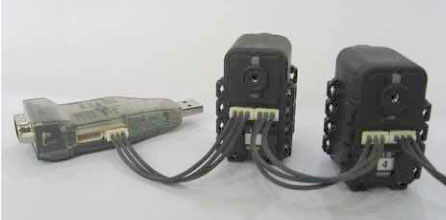
\includegraphics[width=0.5\textwidth]{images/dynamixel.jpg}
\caption{Dynamixel avec la clé de calibration}
\par\end{centering}
\end{figure}

\textbf{Avantages:}
\begin{itemize}
\item Retour de beaucoup d'informations: courant consommé, couple appliqué, vitesse et position,...
\item Configurable
\item Possibilité de les commander avec un seul bus en les connectant en série
\end{itemize}

\textbf{Inconvénients:}
\begin{itemize}
\item Très difficile d'utilisation. Il faut utiliser un connecteur spécial et coûteux pour les débuguer.
\item Plus fragiles que les servomoteurs.
\item Prix (60 euros environ l'unité)
\end{itemize} 

\textbf{Fournisseur:} Robotis et autres revendeurs

\chapter{Système pneumatique}
Nous avons vu jusqu'à présent que des actionneurs électriques. Cependant, il est aussi possible d'utiliser des actionneurs pneumatiques.

\begin{figure}
\begin{centering}
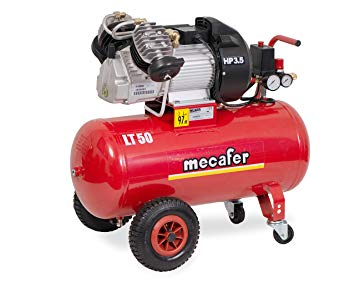
\includegraphics[width=0.4\textwidth]{images/compresseur.jpg}
\caption{Compresseur}
\par\end{centering}
\end{figure}

\textbf{Avantages:}
\begin{itemize}
\item Rapide
\item L'actionneur peut être bloqué sans être endommagé
\end{itemize}

\textbf{Inconvénients:}
\begin{itemize}
\item Nécessité d'une source de pression: compresseur, pompe, cartouche de gaz,...
\item Tout ou rien
\item Risque de fuite ou de bouchage
\end{itemize}

\section{Pompe}
La pompe génère une dépression qui permettra d'aspirer des objets. En général, il s'agit un moteur à courant continu avec un système de soupapes pour générer le vide.

\begin{figure}
\begin{centering}
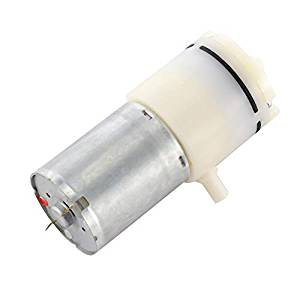
\includegraphics[width=0.4\textwidth]{images/pompeAvide.jpeg}
\caption{Compresseur}
\par\end{centering}
\end{figure}

Les pompes trouvées en ligne sont de qualité très inégales et les spécifications décrites peuvent être fausses. Il ne faut pas hésiter à acheter différents modèles en plusieurs exemplaires. 

\textbf{Fournisseur:}
Les modèles déjà utilisés ont été des pompes à air de 12V trouvées sur Amazon par exemple. Roboshop vend un unique modèle qui est n'est pas mal. Cependant, il est relativement massif et surtout bruyant par rapport aux mini-pompes de 12V d'Amazon, qui font aussi bien le travail.

\subsection{Utilisation}
IL suffit de l'alimenter comme un moteur à courant continu. On peut très bien simplement la brancher à une alimentation 12V ou bien utiliser un pont en H si on souhaite contrôler la quantité d'air aspirer. 

Quand la pompe n'est plus alimenter, elle empêchera légèrement l'air de s'échapper. Ainsi, il ne suffit pas d'arrêter d'alimenter la pompe pour qu'un objet tombe de la ventouse. Pour remédier à ce problème, il y a plusieurs solutions. On peut soit faire un léger trou dans la ventouse ou le tube. La pompe pourra toujours aspirer mais l'objet sera lâché plus rapidement. Sinon, il est possible d'ouvrir le circuit pneumatique avec des valves.

\section{Ventouse}
Les ventouses sont très utilisées pour se saisir d'objets ayant des surfaces relativement plane et lisse.

\begin{figure}
\begin{centering}
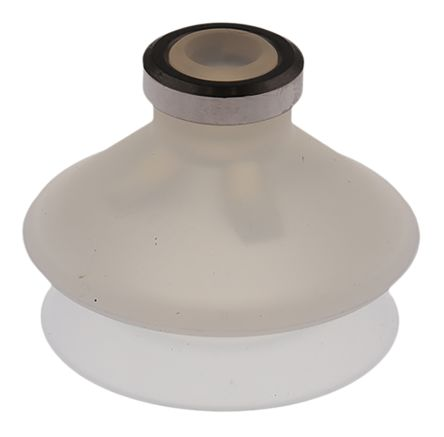
\includegraphics[width=0.4\textwidth]{images/ventouseSoufflet.jpg}
\caption{Compresseur}
\par\end{centering}
\end{figure}

On distinguera surtout 2 types de ventouses: avec et sans soufflet. Le soufflet permet à la ventouse de s'adapter à l'inclinaison de la surface plane de l'objet au moment de le saisir

\textbf{Avantage:}
\begin{itemize}
\item Rapide
\end{itemize}

\textbf{Inconvénients:}
\begin{itemize}
\item Ne fonctionne que sur des surfaces planes
\end{itemize}

\textbf{Fournisseur:} RS

\section{Accessoires et autres}

\subsection{Tubes}

Il faut bien sûr aussi acheter les tubes pour tout relier. Voici les critères importants à regarder quand on achète des tubes:
\begin{itemize}
\item Le diamètre intérieur
\item Le diamètre extérieur
\item Le rayon de courbure (indique à quel point le tube peut être tordu avant de se boucher)
\end{itemize}

Le rayon de courbure est très important. Certaines pompes, même si puissantes, ne pourront pas fonctionner correctement si le tube est trop tordu. C'est pourquoi il est parfois nécessaire d'utiliser des raccords qui font des angles droits.

\textbf{Fournisseur:}Amazon, RS,...

\subsection{Valves}
On peut choisir d'avoir une pompe par ventouse mais cela peut très vite devenir très encombrant. Il faut alors utiliser un système de valves afin de pouvoir bloquer le tube d'une ventouse tout en ouvrant un autre tube. Il existe de vrais valves qu'il est possible d'acheter sur RS. Ces valves seront ensuite actionnées par des servomoteurs. Il est cependant aussi possible de simplement pincer les tubes avec un bras sur un servomoteur. Cela marche aussi très bien.


\chapter{Communication}

\section{Radio}

\begin{figure}[h!]
\begin{centering}
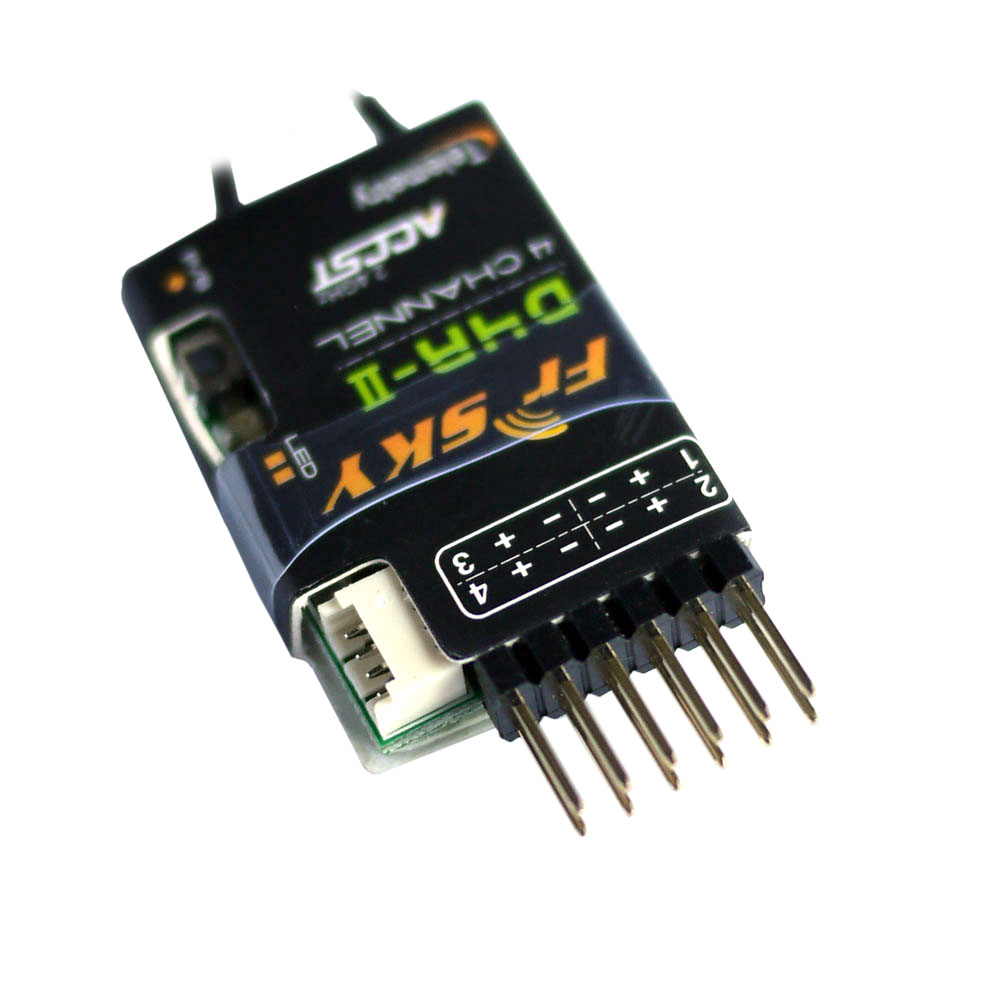
\includegraphics[width=0.5\textwidth]{images/recepteurRadio.jpg}
\caption{Récepteur radio}
\par\end{centering}
\end{figure}

En modélisme, des radiocommandes sont utilisées pour commander avion, bateau ou voiture. De nos jours, la fréquence utilisée en majorité est la 2.4GHz car plusieurs personnes peuvent utiliser cette fréquence sans risquer d'interférences mais avant, des fréquences de l'ordre du MHz étaient utilisées. Ces fréquences dépendent du pays mais en France, on pouvait utiliser 42Mhz et 58Mhz. Ces fréquences ont l'avantage d'avoir une plus grande portée.

\begin{figure}[h!]
\begin{centering}
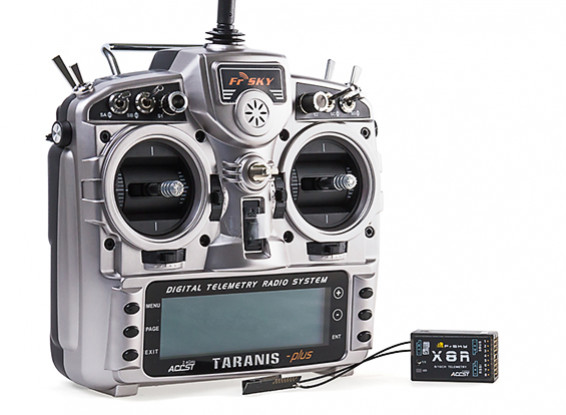
\includegraphics[width=0.5\textwidth]{images/taranis.jpg}
\caption{Radiocommande}
\par\end{centering}
\end{figure}

\section{Bluetooth}

\begin{figure}[h!]
\begin{centering}
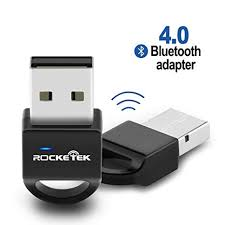
\includegraphics[width=0.5\textwidth]{images/dongleBluetooth.jpeg}
\caption{Adaptateur bluetooth}
\par\end{centering}
\end{figure}

On peut utiliser le Bluetooth pour faire communiquer deux appareils à courte distance. C'est en général ce qui est fait pour transmettre des informations entre 2 Raspberry Pi.

Le Bluetooth utilise 2.4GHz comme le Wifi mais il n'est pas utilisé pour les mêmes applications. Il permet un débit de données plus faibles et à une plus faible portée. En contrepartie, le Bluetooth consomme moins de courant que le Wifi. Les protocoles de communication ne sont aussi pas les mêmes, tout comme les organismes qui gèrent les normes pour le Bluetooth et le Wifi.

\section{Module Xbee}

\begin{figure}[h!]
\begin{centering}
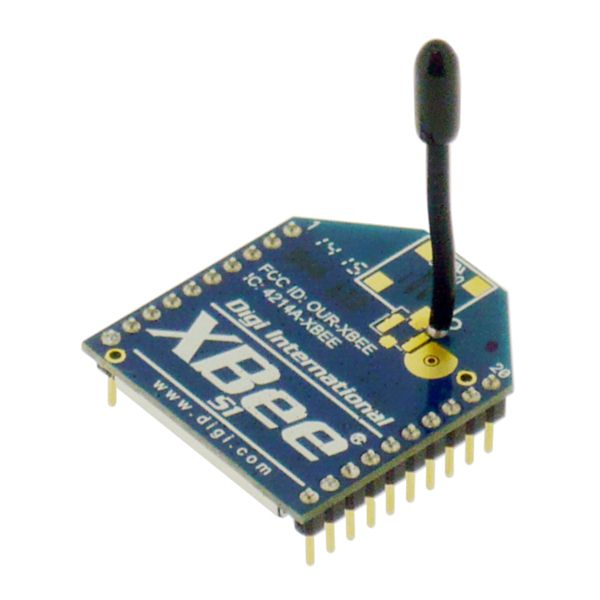
\includegraphics[width=0.5\textwidth]{images/XBee.jpg}
\caption{Module XBee}
\par\end{centering}
\end{figure}

XBee est une marque qui produit des interfaces réseaux. Il en existe une grande diversité. On peut les distinguer par leur architecture réseau, la fréquence utilisée, le type d'antenne et la porté/puissance du signal.

\subsection{Architecture réseau}
Différentes architectures réseaux ont été dévelopées pour les modules Xbee en fonction des besoins.
\subsubsection{•}

\subsubsection{•}

\chapter{Cartes électroniques}

\section{Arduino}

\begin{figure}[h!]
\begin{centering}
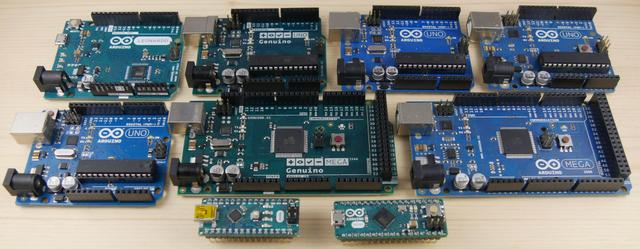
\includegraphics[width=0.5\textwidth]{images/cartesArduino.jpg}
\caption{Différentes cartes Arduino}
\par\end{centering}
\end{figure}

Les cartes Arduino sont les cartes de prototypage les plus populaires de part leur simplicité d'utilisation et leur rapport qualité-prix. La plus répandue est la carte Arduino Uno.

\section{Raspberry Pi}
C'est un micro-ordinateur. Elle est donc beaucoup plus puissante que la Teensy ou les cartes Arduino. Cependant, elle est aussi limité dans ses capacités.

\textbf{Avantages:}
\begin{itemize}
\item Ports USB
\item Wifi et bluetooth intégrés pour la version 3B+
\item Plus de puissance de calcul
\item Possibilités de programmer dans n'importe quel language.
\end{itemize}

\textbf{Inconvénients:}
\begin{itemize}
\item Il est difficile de générer des signals PWM
\item Impossible de lire des signaux PWM
\item Seulement une vrai liaison série disponible et encore. Elle est normalement dédiée au bluetooth mais on peut l'utiliser pour autre chose si on utilise pas le Bluetooth. Il y a aussi une autre pseudo liaison série mais elle est très limitée.
\end{itemize}

\subsection{Ports USB}

\subsubsection{Interface série}

\subsubsection{Courant}

\section{Teensy}
La teensy est en résumé une version miniature d'une carte arduino, en plus puissante. Elle possède notament plus de sortie série. Elle se programme exactement de la même manière qu'une carte arduino.

\section{Node Mcu}
C'est une carte équipé commme la Teensy mais elle a une puce Wifi en plus. C'est la carte de prototypage utilisée pour les applications IoT.



\section{Shield}
Les différentes cartes électroniques ne possèdent pas tous les capteurs ou sorties nécessaires pour un projet. Pour compenser ces problèmes, des Shield ont été créés. Ce sont des extensions des cartes électroniques très faciles d'utilisation. Cela coûte bien sûr moins cher de les faire soit même mais on est certain au moins que c'est fiable avec un shield.

Différents shields:
\begin{itemize}
\item GNSS
\item Servo
\end{itemize}

\chapter{Capteurs}

\section{GNSS}
GNSS (Global Navigation Satellite System)  designe un ensemble de composants reposant sur une constellation de satellites artificiels permettant de fournir à un utilisateur par l’intermédiaire d'un récepteur portable de petite taille sa position 3D, sa vitesse et l'heure.

Il est important de distinguer GPS et GNSS. GPS (Global Positionning System) correspond à la constellation de satellites des Etats-Unis qui appliquent le principe de GNSS. C'est un abus de language.

\textbf{Avantages:}
\begin{itemize}
\item Position absolue
\item Donne aussi la vitesse du véhicule (dans)
\end{itemize}

\textbf{Inconvénients:}
\begin{itemize}
\item La précision des mesures dépend fortement de la qualité du signal. En milieu urbain, les immeubles bloquent certains satellites et peuvent générer des multipaths.
\end{itemize}

\textbf{Fournisseurs:} Ublox, Emlid,...

Il existe différents modes de positionnement par GNSS aujourd'hui dont certains peuvent donner une  précision allant jusqu'au centimètre.

\subsection{NMEA}

\subsection{Mode de positionnement}

\subsubsection{Single}

\subsubsection{PPP}

\subsubsection{Différentiel}


\section{LIDAR}

\begin{figure}[h!]
\begin{centering}
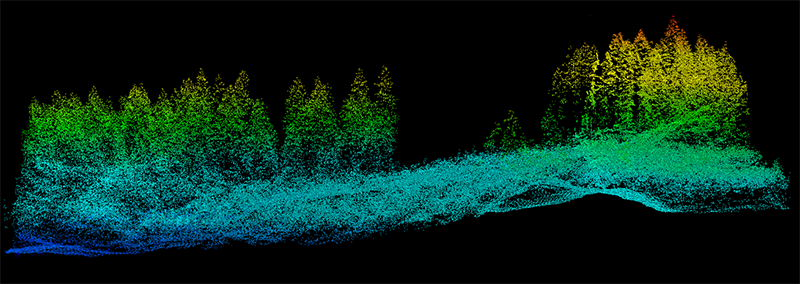
\includegraphics[width=0.5\textwidth]{images/NuageDePoints.png}
\caption{LIDAR de SLAMTEC}
\par\end{centering}
\end{figure}

Acronyme pour Light Detection And Ranging, ce capteur permet de générer un nuage de point de l'environnement qui l'entoure. Le LIDAR fait cela grâce à un laser qui mesure la distance avec un obstacle. Contrairement à un capteur infrarouge actif, le laser du LIDAR est très directif et permet des mesures plus précises. En connaissant la configuration du LIDAR, on connaît la direction du laser et donc la direction de l'obstacle. Les LIDARs que nous utilisons sont font juste des mesures dans un plan mais il existe des LIDARs qui fournissent des nuages de points en 3D.

Un nouveau type de LIDAR est un train de faire son apparition: les Solid State Lidar. Il génère toujours un nuage de points mais il ne fonctionne pas sur le même principe, il n'y pas notamment plus de pièces mobiles. 

\begin{figure}[h!]
\begin{centering}
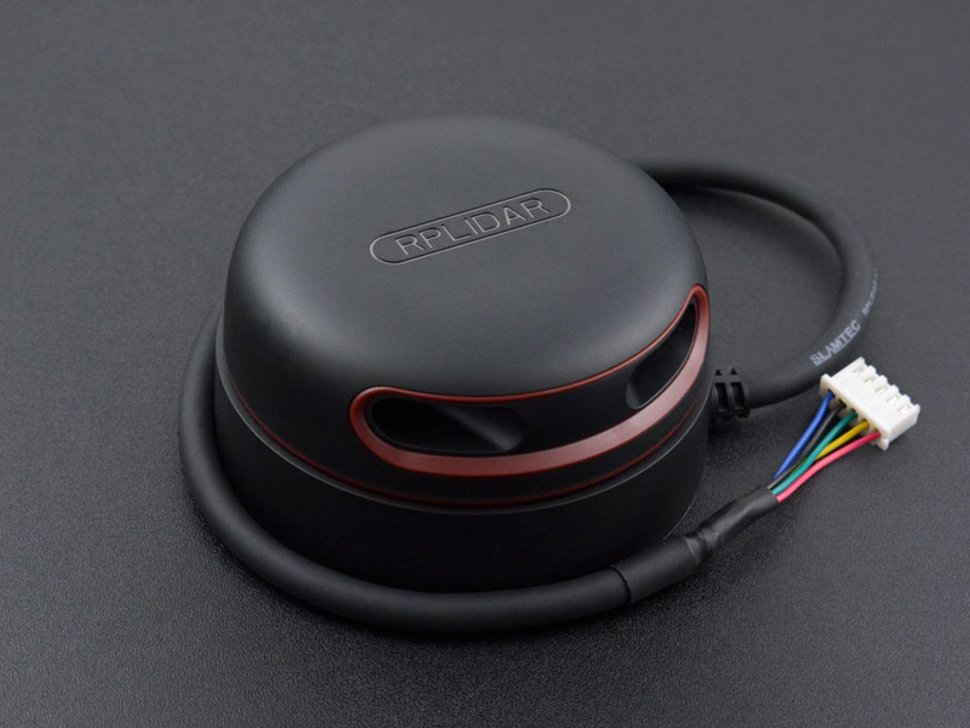
\includegraphics[width=0.5\textwidth]{images/RPLidar.jpg}
\par\end{centering}
\end{figure}

\subsection{Matériel}
\begin{description}
\item[Modèle:] A2M8
\item[Quantité:]2
\item[Fabricant:]Slamtech
\item[Fournisseur:]Robotshop
\end{description}


\subsection{Utilisation}
\begin{description}
\item[Positionnement:]En utilisant des techniques de SLAM, il est possible d'utiliser des balises posées sur le bord du terrain pour obtenir la position et l'orientation du robot. Le problème est que la résolution des LIDAR que Minotaure possède n'est pas suffisante pour détecter les balises partout sur le terrain.
\item[Détection d'obstacles:] Il est possible de détecter les robots adverses à partir du nuage de points. Pour cela, il faudrait faire une détection de blobs, qui correspondraient aux robots.
\end{description}

\section{Ultrason}

\section{Infrarouge}

\begin{figure}[h!]
\begin{centering}
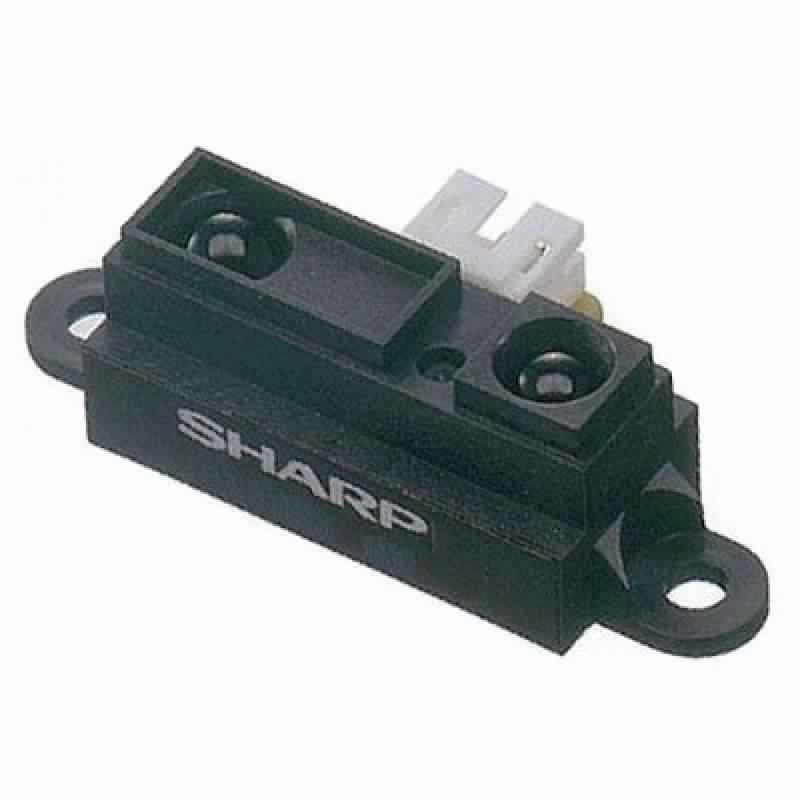
\includegraphics[width=0.5\textwidth]{images/capteurInfrarougeActif.jpg}
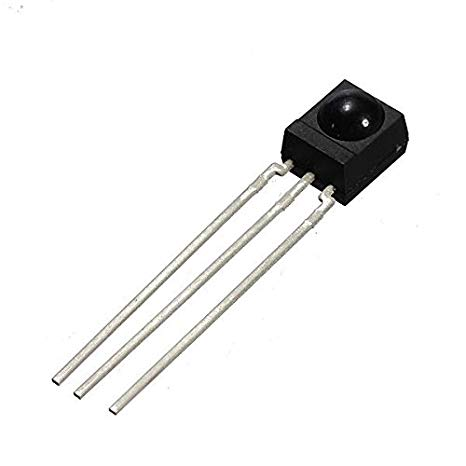
\includegraphics[width=0.5\textwidth]{images/capteurInfrarougePassif.jpg}
\caption{Capteurs infrarouges Actif (gauche) et passif (droite)}
\par\end{centering}
\end{figure}

On distingue 2 types de capteurs infrarouges, les capteurs passifs qui mesurent juste la lumière ambiante et les capteurs actifs qui génèrent aussi des ondes infrarouges. On pourrait aussi parler des caméras infrarouges, mais ce sont simplement des caméras qui mesurent captent les infrarouges en plus des ondes du domaine visible.

\textbf{Avantages:}
\begin{itemize}
\item Peu cher
\item Simple à mettre en oeuvre
\end{itemize}

\textbf{Inconvénients:}
\begin{itemize}
\item Très sensible à la lumière ambiante, les écalairages traditionnels émettent aussi des infrarouges qui peuvent induire le capteur en erreur.
\end{itemize}

\subsection{Utilisation}
Le capteur infrarouge actif est en général utilisé en tant que capteur d'obstacle. En fonction de la quantité d'ondes infrarouges reçues, on peut estimer la distance de l'obstacle. Le problème est que cette quantité varie en fonction de l'écalirage de l'environnement (notamment avec des projecteurs). Pour compenser ce problème, il est nécessaire de calibrer les capteurs infrarouges à chaque lancement.

La phase de calibration peut consister définissant le taux moyen d'infrarouge dans l'environnement en mesurant sur une certaine période ou en redéfinissant la valeur limite.

\section{Capteurs de fin de course}
Comme son nom l'indique, le capteur de fin de course permet d'observer les contacts. Ils sont aussi appelés interrupteurs ou détecteurs de position. Ce sont en soit des interrupteurs poussoirs avec des 

\section{Capteur TOF}
Les capteurs TOF (Time Of Flight) regroupent différents types de capteurs. Ils ont tous en commun la mesure de l'aller-retour d'un signal pour mesurer une distance. C'est en soi le même principe que pour les capteurs ultrasons ou infrarouges. Cependant, on qualifie en particulier 2 capteurs de cette manière: des caméras qui mesurent la profondeur sur le même principe que la Kinect 2 et des capteurs de distance utilisant un laser, à distinguer des LIDAR.

ST a développé un capteur sur ce principe a prix très abordable. La technologie s'appelle FlightSense. De part la précision, la taille et la robustesse de ce capteur, il rend les capteurs ultrasons et à infrarouges obsolètes.

\begin{figure}[h!]
\begin{centering}
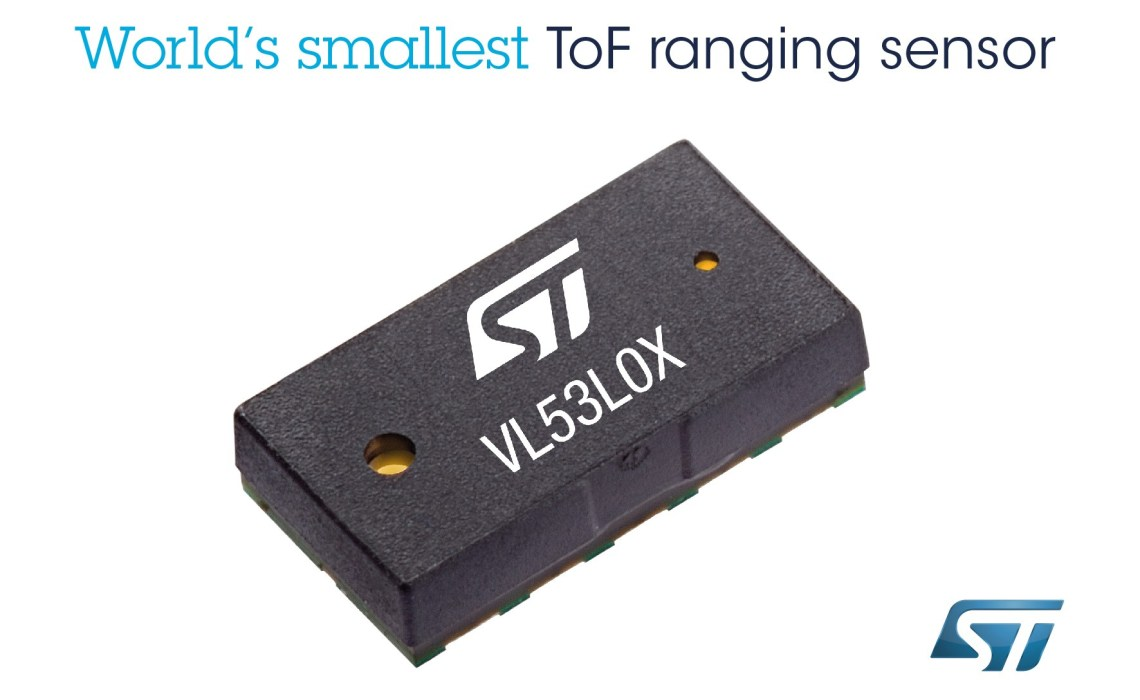
\includegraphics[width=0.5\textwidth]{images/tofSensorST.jpg}
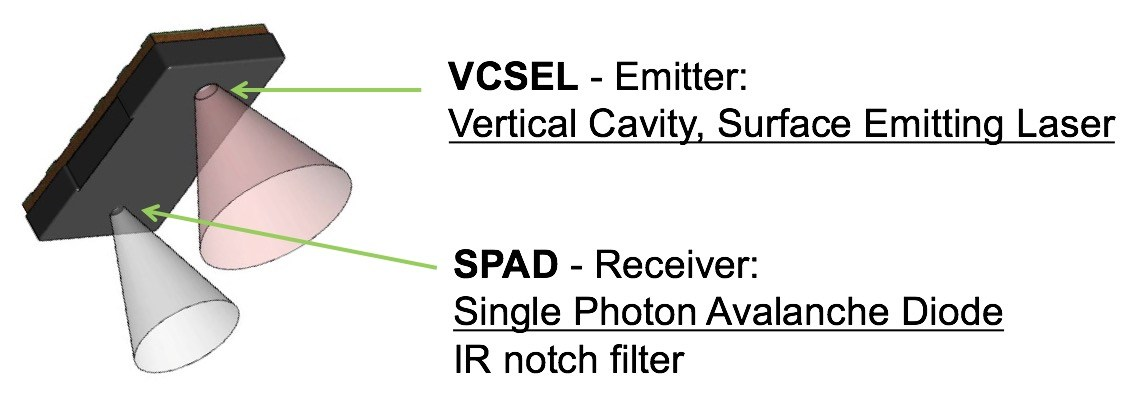
\includegraphics[width=0.5\textwidth]{images/principeFlightSense.jpg}
\caption{Fonctionnement du capteur FlightSense de ST}
\par\end{centering}
\end{figure}

\section{Codeurs incrémentaux}

\begin{figure}[h!]
\begin{centering}
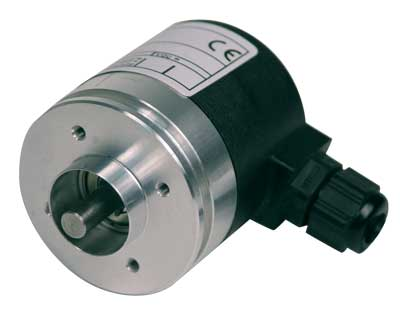
\includegraphics[width=0.5\textwidth]{images/photoCodeurIncremental.JPG}
\caption{Codeur Incrémental}
\par\end{centering}
\end{figure}

Les capteurs incrémentaux mesurent une rotation.

Il existe des codeurs incrémentaux absolus et relatifs. Cependant, les codeurs absolus sont très chers. En effet, chaque position doit avoir son propre code ce qui demande des gravures de très grandes précisions. En général, un codeur incrémental relatif est utilisé avec une phase d'initialisation lors de son démarrage avec un capteur de buté.

\begin{figure}[h!]
\begin{centering}
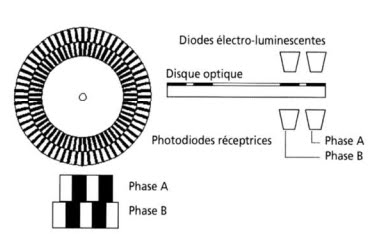
\includegraphics[width=0.5\textwidth]{images/codeurIncremental.jpg}
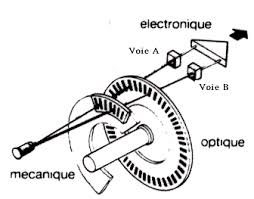
\includegraphics[width=0.5\textwidth]{images/schemaCodeurIncremental.jpeg}
\caption{Schema de codeurs incrémentaux}
\par\end{centering}
\end{figure}

\section{Caméra}
Il existe 2 types majoritaires de capteurs photographiques: CDD et CMOS. Cependant, un  nouveau type de capteur fait se popularise dans le milieu de la robotique: DVS (Dynamic Vision Sensor).

\begin{figure}[h!]
\begin{centering}
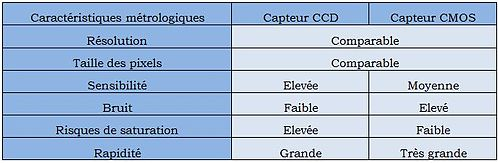
\includegraphics[width=0.5\textwidth]{images/differenceCDD_CMOS.png}
\caption{Différences entre capteurs CDD et CMOS}
\par\end{centering}
\end{figure}

Pour plus d'information sur la différence technique entre CMOS et CDD: \url{https://www.photoniques.com/articles/photon/pdf/2015/06/photon201579p39.pdf}

Pour plus d'information sur les capteurs DVS: \url{http://rpg.ifi.uzh.ch/docs/EventVisionSurvey.pdf}

\subsection{CDD}

CDD signifie Charged Coupled Device. C'est un capteur avec de meilleurs performances mais beaucoup plus coûteux. Il est notamment utilisé dans l'industrie du cinéma. Il consomme aussi plus de puissance ce qui fait qu'il chauffe aussi plus rapidement. Il faut le refroidir à moins de voir apparaître des signaux parasites.


\subsection{CMOS}

CMOS signifie Complementary Metal Oxyde Semiconductor. C'est la technologie la plus récente. Au départ, les CDD possédaient de meilleurs performances mais de plus en plus, cet écart se réduit. Le facteur le plus distinctif entre les 2 caméras est la sensibilité à la lumière. Dans un endroit peu éclairé, il y aura beaucoup de bruit sur une image prise avec un capteur CMOS.

\subsection{DVS}
Un nouveau type de caméra fait son apparition: DVS (Dynamic Vision Sensor). Ce type de caméra n'enregistre pas une image à chaque pas de temps. Elle suit le même principe que les récepteurs lumineux dans nos yeux et enregistrement seulement les variations de luminosité. Ces caméras ont beaucoup de potentiel. En effet, puisque seulement la variation est enregistrée, il n'y a pas d'informations redondantes et les programmes peuvent être plus rapides. De plus, ces caméras sont plus aptes à enregistrer les mouvements rapides de part leur nature. Contrairement aux capteurs CDD et CMOS, il n'y a pas " de perte d'inforamtion" entre 2 images. Problème: les DVS coûtent très chères et ont encore une très faible résolution pour le prix demandé. Cependant, en terme d'application pour la robotique, c'est le futur.

\subsection{Matériel}
En général, des PiCameras sont utilisés pour les projets demandant de la vision. Il faut distinguer les 1ère versions (V1) et les 2ème versions (V2). Il existe aussi des Picameras qui captent aussi les infrarouges afin d'avoir une vision nocturne (une lampe infrarouge est cependant nécessaire en plus). Dans la plupart des cas, cela suffira.

\begin{figure}[h!]
\begin{centering}
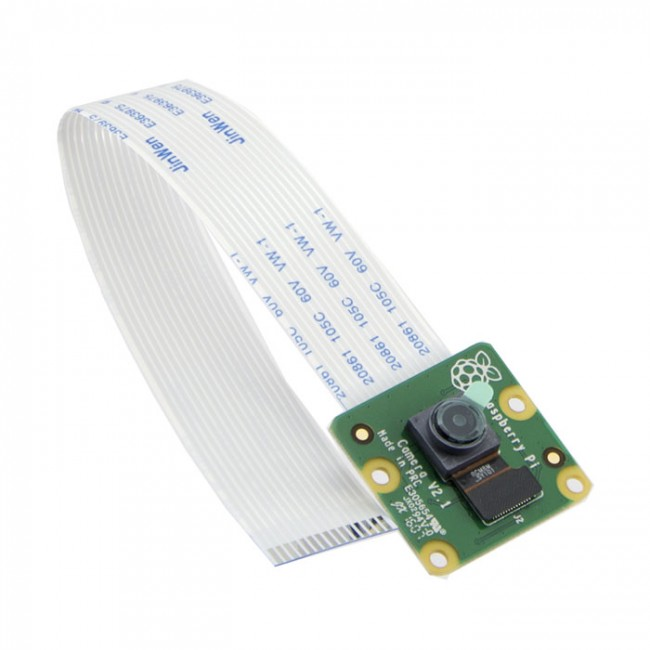
\includegraphics[width=0.5\textwidth]{images/picamera.jpg}
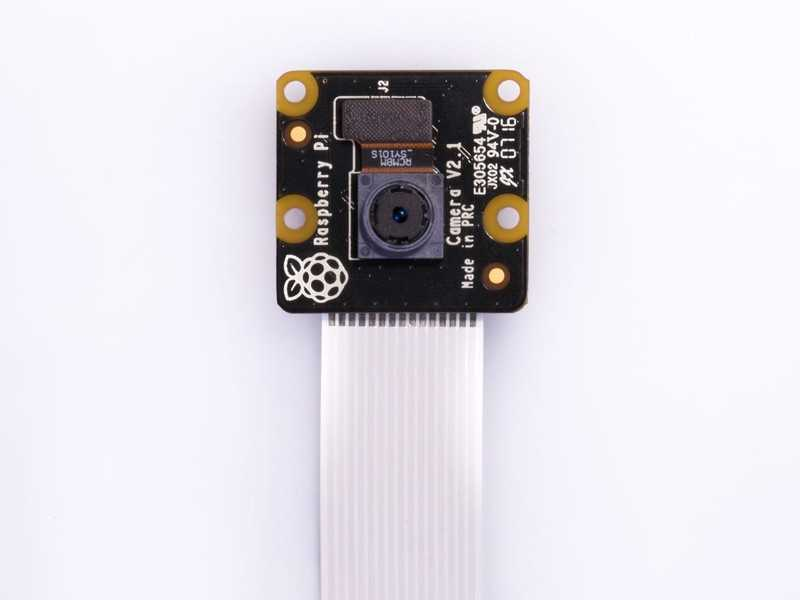
\includegraphics[width=0.5\textwidth]{images/picameraNoir.jpg}
\caption{Picamera et Picamera Noir}
\par\end{centering}
\end{figure}

\subsection{Utilisation}
La picamera est facilement utilisable avec Python. Du C++ peut aussi être utilisé pour la commander mais c'est beaucoup plus complexe.

Toutes les informations nécessaires sont présentes sur ce site: \url{https://picamera.readthedocs.io/en/release-1.13/}

\textbf{Possibilités:}
\begin{itemize}
\item Choisir la résolution de l'image et le FOV (Field Of View)
\item Encodage utilisé
\item Paramètre caméra (saturation, nombre d'image par seconde si on prend une vidéo, ...)
\end{itemize}


\subsection{Autres}
Intel a développé des caméras avec des cartes intégrés pour exploiter les données des caméras directement. La marque s'appelle RealSense.

\subsubsection{T265}
Stéréo caméra avec des lentilles fisheyes. Elle ne mesure pas la profondeur d'une image de manière innée. Il faut exploiter les caméras avec OpenCV pour cela. Elle est par contre spécialisé dans le SLAM. La T265 peut mesurer son déplacement et son attitude avec une très grande fiabilité et précision.

\begin{figure}[h!]
\begin{centering}
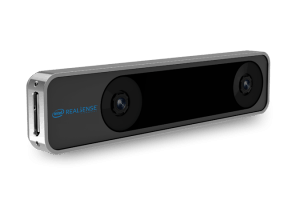
\includegraphics[width=0.5\textwidth]{images/T265.png}
\caption{T265 d'Intel RealSense}
\par\end{centering}
\end{figure}

\subsubsection{D435}
C'est une stéréocaméra infrarouge qui permet de mesurer la profondeur d'une image. Il y a aussi une caméra RGB pour avoir une image en couleur en plus.

\begin{figure}[h!]
\begin{centering}
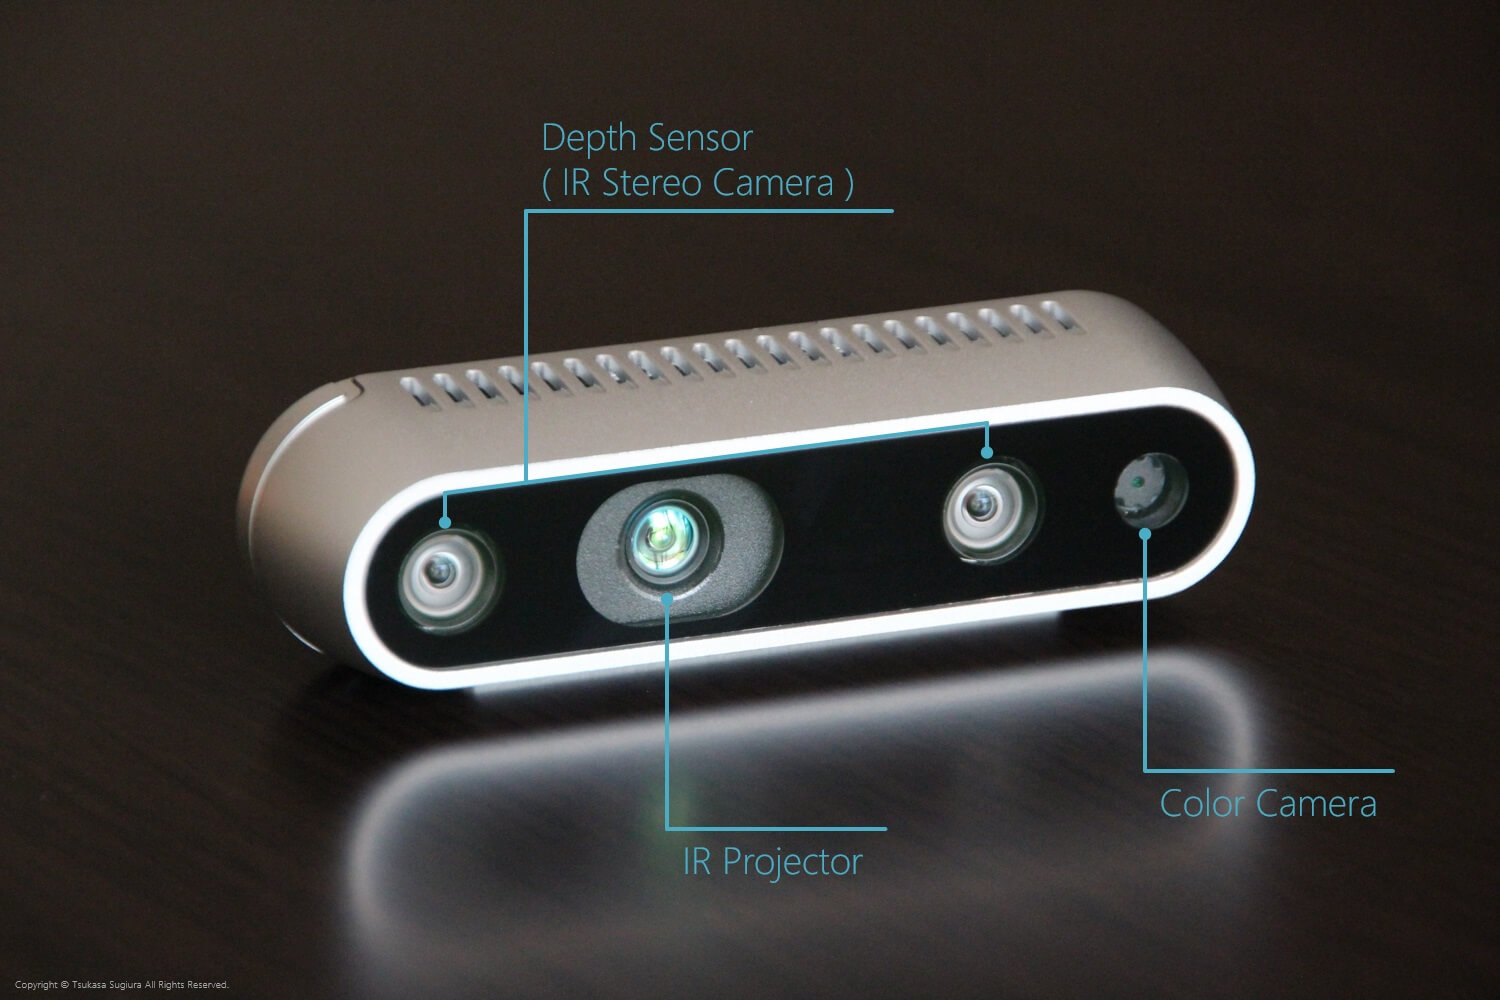
\includegraphics[width=0.5\textwidth]{images/D435.jpg}
\caption{D435 d'Intel RealSense}
\par\end{centering}
\end{figure}


\chapter{Alimentation}

\section{Batterie}
Il existe 2 types majoritaires de batterie chimique. Les Lithium Polymère (LiPo) et les Nickel Mercure (Nimh).

\subsection{Lipo}
Ces batteries présentent la meilleure densité énergétique. Cependant, elles sont aussi très dangereuses. Elles peuvent en effet exploser et provoquer un feux chimique difficilement arrêtable.

Les choses suivantes peuvent causées l'explosion d'une LiPo.
\begin{itemize}
\item Mouillée
\item Percée
\item Recoit un choc
\item Laissée au soleil
\item Court-circuit
\end{itemize}

Si jamais la LiPo est bombée ou a des bosses, il faut absolument s'en débarasser. En attendant, la meilleure solution est de la placé dans un sceau en métal ou sur une surface non-inflammable (pierre, métal, ...). Ce type de batterie doit être jeté à la déchèterie dans la section réservée pour.

\subsubsection{Les critères de sélection}
\begin{description}
\item[Taux de décharge:]Indique combien d'ampère la batterie peut fournir en continu. Le taux de décharge est mesuré en C. Il faut appliquer la formule: $Courant Max = C * \frac{Capacité de la batterie (mAh)}{1000}$. Le taux de décharge est souvent surestimé. Prendre un taux de décharge trop petit détériora la batterie est celle-ci pourra gonfler.
\item[Nombre d'élément:]Correspond à la tension de la batterie. C'est mesuré en S.
\end{description}

\subsubsection{Les bonnes marques}
\begin{itemize}
\item Tattu
\item Turnigy
\item Zippy
\end{itemize}
Liste non-exhaustive.

\subsection{Nimh}
Les batteries Nimh sont moins fragiles que les batteries Lipo. Cependant, elles ont une plus faible densité énergétique.

\subsection{Chargeur}
Les différents types de batterie ne se chargent pas de la même façon. Il y a un mode pour chaque sur le chargeur. Il faut aussi surveiller le taux de charge.

\begin{figure}[h!]
\begin{centering}
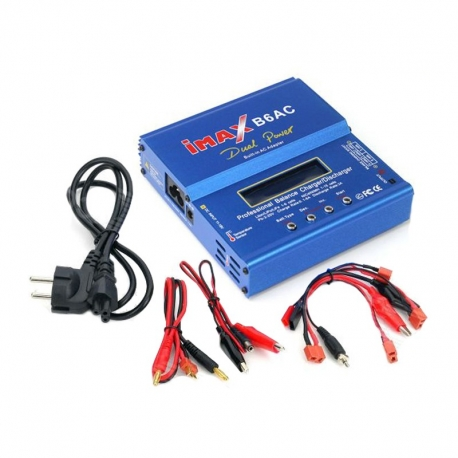
\includegraphics[width=0.5\textwidth]{images/chargeurBatterie.jpg}
\caption{Chargeur de batterie}
\par\end{centering}
\end{figure}

Pour les Lipo, il faut aussi brancher la prise d'équilibrage. Ce n'est pas obligatoire mais cela permet de prolonger la durée de vie de la batterie. En effet, au fur et à mesure des différents cycles de charge/décharge, les éléments de la Lipo ne vont pas avoir tous la même tension. La prise d'équilibrage permet d'empécher cela.

Les batteries ont en général un taux de recharge de 1C. Le courant pour recharger la batterie est à définir sur le chargeur. Il faut appliquer la même formule que pour le courant de taux de décharge.

\section{Adapter l'alimentation}

\subsection{BEC}
Le BEC (Battery Eliminator Circuit) permet de délivrer une tension. Ce circuit appartient à l'électronique de puissance.

Dans la plupart des ESC de nos jours, un BEC est intégré et fournis du 5V.

Il faut distinguer plusieurs BEC:
\begin{description}
\item[BEC:]Les BEC de base. Ils utilisent des régulateurs de tension comme expliqué dans la section suivante.
\item[SBEC:]Switch BEC. Ce sont les BEC qui convertissent toutes la puissance. Le Switch fait référence à comment le signal entrant est traité pour être transformé. Ils utilisent un convertisseur Buck.
\item[UBEC:]Universal BEC. C'était/c'est une marque de BEC. Il fonctionne sur le même principe que les SBEC, mais il peut y en avoir qui fonctionne encore avec des régulateurs de tension.
\end{description}

\subsubsection{Régulateurs de tension linéaire}
Les régulateurs permettent comme les BEC de fournir une tension inférieur à la tension d'alimentation. Cependant, contrairement à un BEC, toute la puissance n'est pas convertie. Une grande partie est perdue par effet joule. C'est pourquoi il ne faut l'utiliser que quand la puissance à dissiper est faible ($P_{dissipée} = (V_{entrée} - V_{sortie})*I$).

\textbf{Inconvénients:}
\begin{itemize}
\item Pas efficace, la tension a dissipé l'est sous la forme de chaleur
\item Cesse de d'alimenter en tension si la température dépasse un certain seuil
\item Chauffe beaucoup si il y a beaucoup de puissance à dissiper
\end{itemize}

\textbf{Avantages:}
\begin{itemize}
\item Simple à mettre en oeuvre
\item Peu cher (de l'ordre de la dizaine de centimes)
\end{itemize}


\subsection{Convertisseur Buck}
C'est ce qu'il faut choisir quand il y a beaucoup de puissance à dissiper (tous les cas sauf quand il faut alimenter un micro-contrôleur en 3.3V en partant de 5V par exemple).

\textbf{Inconvénients:}
\begin{itemize}
\item Prix de l'ordre de l'euro
\item Utilise une bobine donc peut être source d'interférences électromagnétiques
\end{itemize}

\textbf{Avantages:}
\begin{itemize}
\item Fort rendement
\end{itemize}

\chapter{Composants électroniques}

\section{Fusible}

\subsection{PTC}

\subsection{Fusible réinitialisable}

\subsection{Thermistor}

\part{Programmation}

\chapter{Raspbian}

\section{Le Set up}
En règle général, il n'y aura pas d'écrans, de claviers ou de souris à disposition pour pouvoir utiliser directement la raspberry pi avec son ordinateur. Pour controurner ce problème, Matthieu Vignes(P14) a créé une configuration spéciale de l'image Raspbian.  Elle fait en sorte que dès le premier démarrage, la raspberry pi émet son propre réseau wifi sur lequel il est possible de se connecter pour pouvoir utiliser la raspberry pi.

La méthodologie pour créer cette image est disponible sur son Github:
\url{https://github.com/matthieuvigne/MiAM_eurobot2019/tree/master/ConfigRPi}

\begin{description}
\item[Windows:]Il faut installer Putty pour avoir accès au terminal de la raspberry pi. Sinon, il est possible d'avoir accès à la GUI avec VNC viewer.
\item[Linux:]Il faut utiliser les lignes de commandes.
\end{description}

\begin{description}
\item[sshfs:]Monter sur son système de fichier, un autre système de fichier distant, à travers une connexion SSH . En gros, il est possble d'avoir accès sur l'ordinateur à tous les fichiers de la raspberry pi. Les modifications sur l'ordinateur seront aussi réalisées sur la raspberry pi.
\item[ssh:]Créé une liaison SSH avec la raspberry pi, ce qui permet d'avoir accès à son terminal.
\item[scp:]Copie les fichiers de la raspberry pi à l'ordinateur et vice-versa par liaison SSH. 
\end{description}

Matériel utile:
\begin{description}
\item[Clef USB Wifi:]Permettra à l'ordinateur de se connecter à 2 réseaux Wifi en même temps: Celui de la raspberry pi et à une connection internet.
\item[Cable ethernet:]La raspberry Pi utilise déjà le wifi pour communiquer avec l'ordinateur. Il est alors nécessaire d'utiliser le cable ethernet pour pouvoir réaliser des mises-à-jours logiciel. Il faut pour cela faire un partage de connection par ethernet avec l'ordinateur.
\end{description}


\section{Le système d'exploitation}
Raspbian est un système d'exploitation basé sur Linux. Il est possible d'installer 2 versions sur la Raspberry Pi: la version lite (sans interface graphique), la version graphique (beaucoup plus lourde et gourmande en ressource). En règle générale, il es préférable d'installer la version Lite, cela laissera plus de puissance de calcul pour les programmes qui tourneront dessus.

\subsection{Les commandes utiles}
\begin{description}
\item[cd:] Changer de répertoire. Taper juste "cd" permet de répertoire /home/user. Pour accéder à la racine, il faut taper "cd /".
\item[ls:] Liste tous les fichiers dans un répertoire
\item[mkdir:] Crée un répertoire
\item[nano:] Affiche le contenue texte d'un fichier et permet de le modifier.
\item[vim:] Même chose que nano mais en plus puissant et moins intuitif.
\item[chmod:] Change les permissions d'un fichier. Certains fichiers ne pourront pas être modifiés ou lancés car l'utilisateur n'aura pas le droit.
\item[apt install:] Installe une librairie.
\item[apt upgrade:] Télécharge les versions actuelles des librairies.
\item[apt update:] Met-à-jour les librairies.
\end{description}

Pour lancer un programme binaire, il faut "./programme"

\subsection{Utiliser une clef USB}
Une clef USB ne peut pas être utilisé directement avec Linux, il faut la monter. Dans les OS avec interface graphique, cette étape se fait automatiquement mais pas si on utilise la verison Lite de Raspbian.

Trouver le périphérique:
lsblk

Le périphérique SUB apparaîtra dans le dossier /dev en général avec le nom sdb1. Il faut alors créer un dossier dans /media qui correspondra à notre clef USB.

sudo  mkdir /media/usb 

sudo mount /dev/sdb1 /media/usb

sudo umount /media/usb

\chapter{Le code}

Quel langage utilisé?

\section{Python}
Python, le langage que tout le monde maîtrise normalement après la prépa. Il est très facile de faire du prototypage avec. C'est d'ailleurs avec ce langage qu'il faudra tester de nouvelles choses. Cependant, en tant que langage interprété il est beaucoup plus lent que les langages compilés (C/C++).

En général, c'est le langage utilisé lors de la phase de prototypage. Une fois le principe vérifié, le code embarqué est plutôt en C ou C++.

\section{C/C++}
En tant que langages compilés, ils sont beaucoup plus rapides que Python. Cependant, ils sont aussi beaucoup plus complexe d'utilisation.

\subsection{Cross-compilation}
Il est possible de compiler les programmes en C et C++ sur la raspberry pi mais cela prends beaucoup de temps en raison du manque de puissance de calcul (de l'ordre des minutes). Cependant, une fois compiler une première fois, le compilateur ne devra recompiler que les fichiers modifiés. La compilation prendra alors moins de temps. 

En raison de l'architecture différente des processeurs sur l'ordinateur et sur la Raspberry Pi (ARM), il n'est pas possible de compiler les programmes sur l'ordinateur puis de les copier sur la Raspberry Pi. Il est cependant possible de simuler l'environnement de la raspberry pi pour la compilation sur ordinateur en utilisant la cross-compilation.

\chapter{Traitement de signaux GNSS: RTK Lib}

RTK Lib est un ensemble de programmes créés pour pouvoir exploiter et analyser les signaux obtenus à partir de récepteurs GNSS. Il existe un ensemble avec une interface graphique utilisable sous Windows. Il existe aussi une version UI utilisable sous n'importe quel système d'exploitation après avoir compiler les programmes en C.

Une branche a été créé à partir de RTK Lib: RTK Lib Explorer. Cette branch a été optimisée pour certains récepteurs et fonctionne en général mieux(en tout cas dans les cas vus).

\chapter{Traitement d'images: OpenCV}

OpenCV est la bibliothèque par excellence pour tout ce qui concerne le traitement d'images.

\section{Systèmes de couleur}
De part la manière dont nous voyons le monde, nous utilisons en général le système RGB pour décrire les couleurs. Cependant, ce n'est pas toujours le système de couleur le plus efficace pour étudier des images. En effet, certains éléments ressortiront plus dans un certain système de couleur. Par exemple, les feux de forêt sont plus distinct avec la luminescence du système LUV qu'avec le rouge de RGB.

\begin{figure}[h!]
\begin{centering}
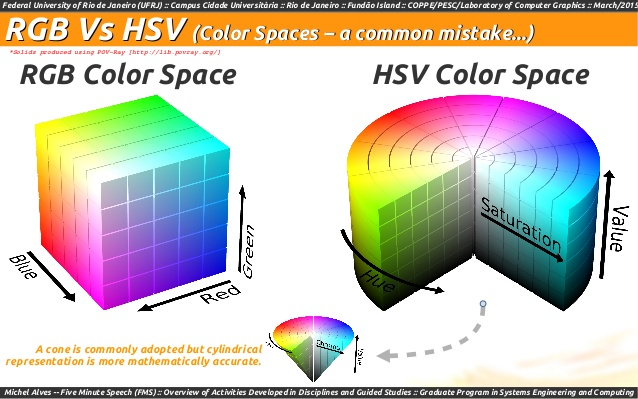
\includegraphics[width=0.4\textwidth]{images/RGB_HSV.jpg}
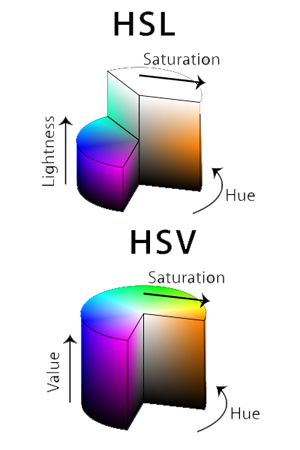
\includegraphics[width=0.4\textwidth]{images/HSL_HSV.jpg}
\caption{Systèmes de couleur}
\par\end{centering}
\end{figure}

\section{Odométrie visuel}
Ces algorithmes permettent de mesurer le déplacement effectué entre 2 images. On peut utilisé une seule ou même deux caméras.

\url{https://link.springer.com/article/10.1186/s40064-016-3573-7}

\section{Vision stéréoscopique}
A partir de deux caméras dont on connaît la position relative, il est possible d'obtenir la profondeur de l'image. Cependant, cette méthode pour obtenir la profondeur est très sensible à différents paramètres tels que la calibration des caméras et la distance entre les caméras. Par ailleurs, la carte de profondeur générée est très approximative. Si on veut vraiment mesurer la profondeur d'une image, on utilisera plutôt une caméra infrarouge telle que la Kinect ou la Intel Realsense D435.

\begin{figure}[h!]
\begin{centering}
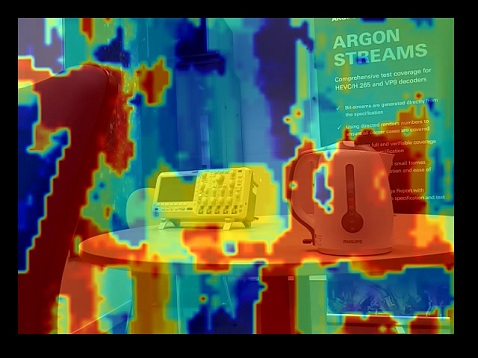
\includegraphics[width=0.6\textwidth]{images/depthMapStereo.jpg}
\caption{Profondeur d'image avec des stéréos caméras}
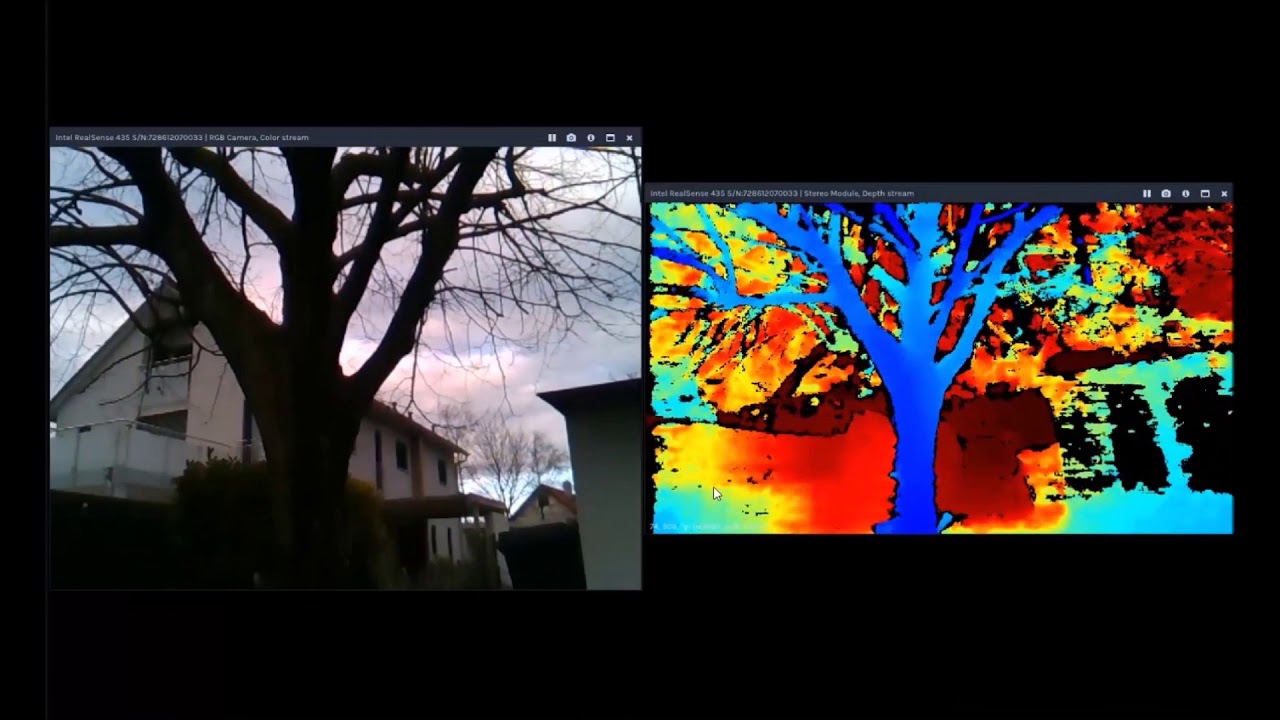
\includegraphics[width=0.6\textwidth]{images/depthMapRealSense.jpg}
\caption{Profondeur d'image avec RealSense D435 utilisant une caméra infrarouge}
\par\end{centering}
\end{figure}

\chapter{ROS}

ROS est une sorte de système d'exploitation pour la robotique.

Pourquoi l'utiliser:
\begin{itemize}
\item Une grande communauté
\item Beaucoup de bibliothèques déjà développées
\item Code beaucoup plus modulable
\item Possibilité de programmer un C/C++ ou en python (autres langages supportés aussi de manière non officielle)
\item Il est très souvent utilisé dans le milieu de la robotique
\end{itemize}

Cependant, ROS demande une certaine prise en main. Pour apprendre à l'utiliser, il a plusieurs solutions. Personnellement, je conseille ce livre disponible en version PDF\href{https://community.robotsource.org/t/download-the-ros-robot-programming-book-for-free/51}{"ROS Robot Programming Book"} . Il rassemble tout ce qui est nécessaire de savoir.

Cependant, pour avoir de la pratique, investir dans la plateform \href{https://www.robotigniteacademy.com/en/}{IgniteAcademy} est une très bonne idée. Un abonnement au mois coûte 39 euros. Je l'ai essayé et ça vaut vraiment le coût.

\chapter{Utilisation d'un Git}
Un Git est très pratique pour coder. Il permet travailler à plusieurs sur un même projet et surtout il permet de gérer l'évolution du code.

Il existe plusieurs services qui propose hébergements en ligne: Github, Gitlab,... Minotaure utilise GitHub.

\section{Documenter}
Il existe deux manières de documenter le code sur GitHub. On peut soit écrire des fichiers README.md ou rédiger des pages Wiki. L'utilisation de l'un ou de l'autre va seulement changer ou trouver l'information ainsi que son organisation. En effet, il est seulement possible d'avoir un fichier README.md par répertoire mais on avoir autant de pages wiki organisées comme on veut.

\subsection{Utilisation de fichier README.md}
Il est possible dans chaque répertoire de créer un fichier README.md. Il s'agit d'un fichier texte mis-en-forme (Markdown Documentation). Ainsi, quand le répertoire sera ouvert sur le site Github, le texte mis-en-forme sera affiché automatique sous les fichiers du répertoire.


\subsection{Utilisation du Wiki}
Chaque github offre la possibilité de créer son propre wiki. Il est possible d'agencer les pages wiki comme on le souhaite. La hiérarchie est la même que pour des fichier normaux: "repertoire1/repertoire2/pageWiki3" par exemple (c'est ce qu'il faut écrire comme nom de page lors de sa création).

\begin{figure}[h!]
\begin{centering}
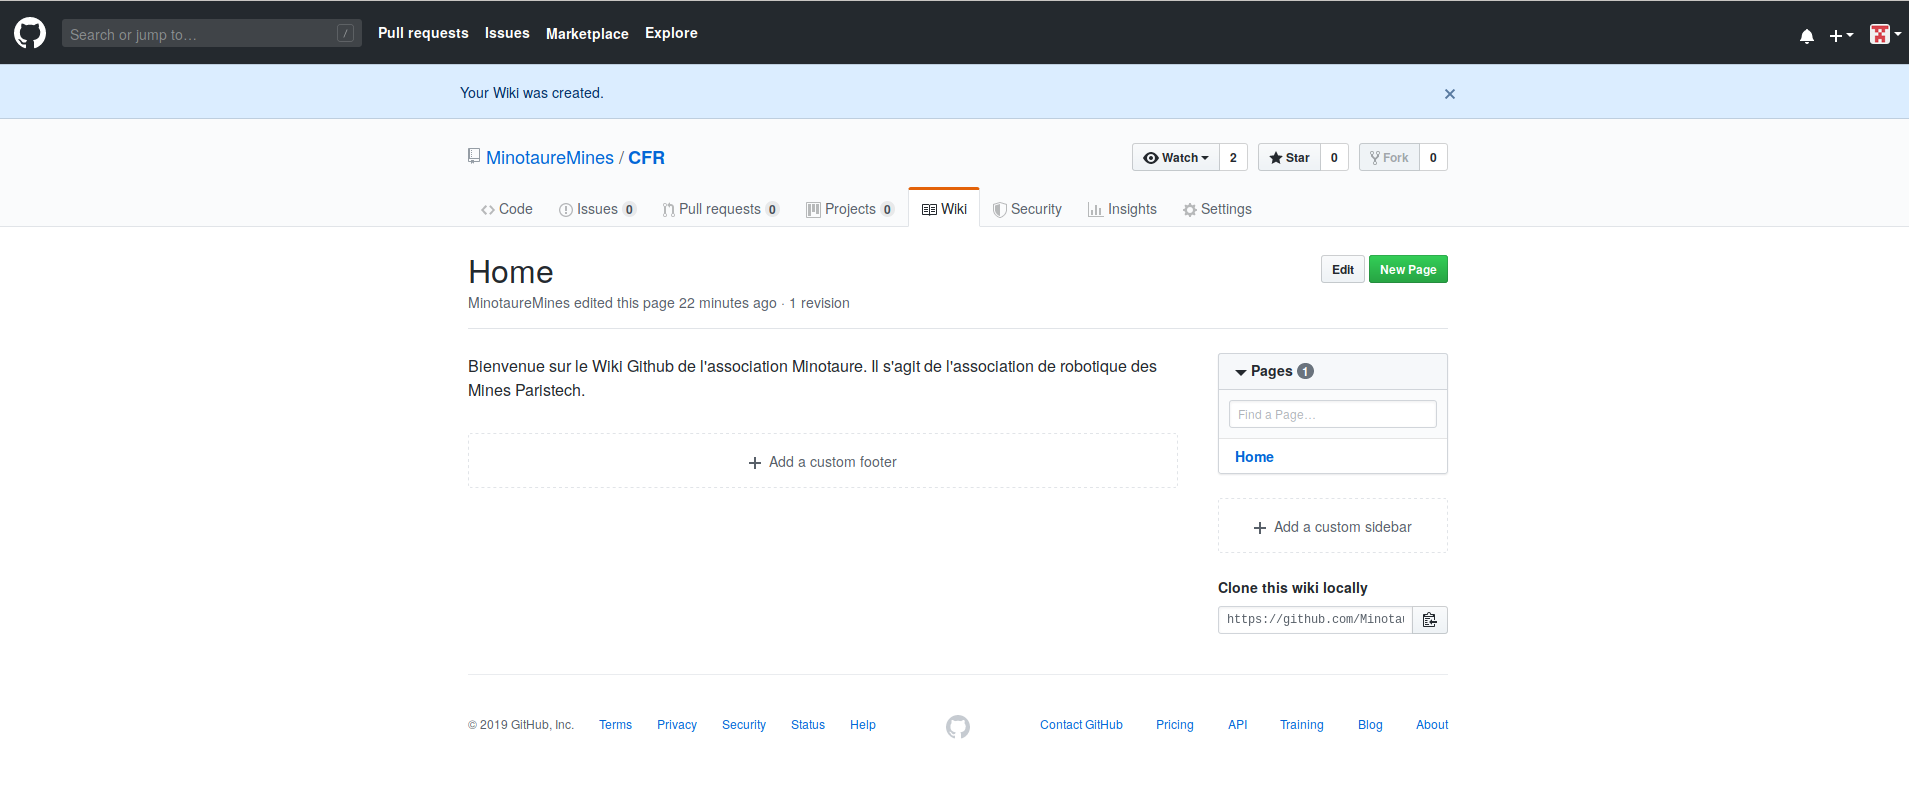
\includegraphics[width=0.4\textwidth]{images/wikiGit.png}
\caption{Wiki du Git}
\par\end{centering}
\end{figure}

\subsection{Mise en forme du texte}
Il est possible de mettre en forme le texte dans le wiki ou le README. Pour cela, le markup language est utilisé. Il est très simple à utiliser et rend les choses lisibles.

\begin{description}
\item[Titres:] Il faut mettre \# avant le titre (Attention de ne pas oublier un espace entre le \# et le titre). Le nombre de \# indique l'importance du titre: \# pour les titres les plus importants, \#\#\#\#\#\# pour les moins importants.
\item[Liste:] Les listes sont indiquées par des *, + ou - au début de la ligne pour chaque élément.
\item[Italique:] *texte en italique* ou \_texte en italique\_
\item[Gras:] **texte en gras** ou \_\_texte en gras\_\_
\item[Barré:]~~texte barré~~
\item[Liens:] [Nom du lien](lien url)
\item[Images:] ![nom image](path vers image ou url)
\item[Code:] ```languageDeProgrammation   ```
\end{description}


\section{Méthodologie}

\subsection{Bases}
\begin{enumerate}
\item Avant de commencer, il faut récupérer la dernière version disponible du code.
\item Une fois satisfait avec les modifications réalisées sur un fichier et avoir vérifier que cela fonctionne, on commit (enregistre) la nouvelle version (on n'enregistre que très rarement un code qui ne fonctionne pas). Il faut mettre un commentaire au commit afin de garder une trace des modifiations réalisées.
\item Quand on a finit de travailler sur le code, on push (sauvegarde)  les modifications sur le serveur.
\end{enumerate}

Il est très important de qu'un commit corresponde à une seule modification afin de garder une trace des modifications. Cela permettra un débugage plus rapide par la suite. Commiter plusieurs modifications d'un seul coup est à proscrire!

\subsection{Branches}
Parfois, on veut tester plusieurs idées pour améliorer un code. Pour éviter de tout mélanger et d'avoir plusieurs fichiers qui font presque la même chose, on utilise des branches. Il s'agit d'une version alternative de tout le code qu'il est possible de développer en parallèle de la branche principale. Une fois satisfait des améliorations réalisées, on peut merger (fusionner)la branche au master (branche principale). Le code des deux branches est alors fusionner.

\begin{figure}[h!]
\begin{centering}
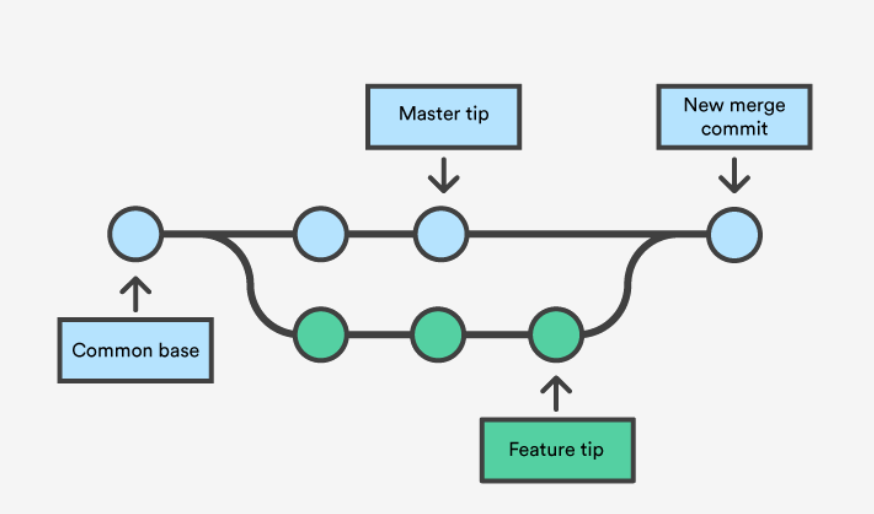
\includegraphics[width=0.4\textwidth]{images/gitBranches.png}
\caption{Principes des branches sur Git}
\par\end{centering}
\end{figure}

\section{Commandes}
Voici une liste non-exhaustive des commandes git de base. Chaque commande possède des options d’utilisation qui ne sont pas décrites ici. Pour plus d'information, chercher sur internet.


\begin{description}
\item[git config:] Définit les paramètres utilisateurs comme le nom d'utilisateur et l'adresse mail.

git config –global user.name “[name]”

git config –global user.email “[email address]”

\item[git init:]Initalise un répertoire git.

git init [repository name]

\item[git clone:]Clone un répertoire sur internet à partir du lien url de celui-ci.

git clone [url]

\item[git add:]Enregistre les modifications des fichiers en vu d'un prochain commit.

git add [file]

\item[git commit:] Commit les modifications enregistrées avec git add.

git commit -m "[Commentaires]"

git commit -a (Commit tous les fichiers modifiés et déjà suivi par git, pas besoin d'utiliser git add)

\item[git reset:]

git reset [file] (Enlève le fichier des fichiers à commit)

\item[git staus:] Liste tout les fichiers modifiés qui n'ont pas été enregistrés pour le commit

\item[git rm:] Efface un fichier

git rm [file]

\item[git log:] Montre l'historique des commits dans la branche locale.

\item[git push:] Sauvegarde les commits en ligne.

git push origin master (Si tu travailles sur la branche principale)

\item[git pull:] Met-à-jour les fichiers locaux par rapport à leur version en ligne.

\end{description}

\chapter{Protocole de communication}

\section{Filaire}

Pour faire communiquer différents appareils électroniques entre eux, il existe plusieurs méthodes.

\subsection{PWM}
Il ne s'agit pas d'un protocole de communication à part entière. C'est cependant la méthode la plus basique et facile à comprendre.


\begin{figure}[h!]
\begin{centering}
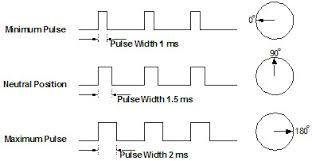
\includegraphics[width=0.5\textwidth]{images/PWMservo.jpeg}
\caption{Signal PWM pour contrôler un servomoteur}
\par\end{centering}
\end{figure}

La durée d'un signal PWM (Pulse Width Modulation) est proportionnelle à la commande. En général, la fréquence est de 50 Hz pour les servomoteurs mais elle peut être différente pour d'autres applications.

C'est le signal utilisé pour contrôler aussi les ESC des moteurs brushless et beaucoup de capteurs basique codent l'information en PWM.

\subsubsection{Lire signal PWM}
Générer un signal PWM est relativement simple. Les lire est une autre paire de manches. On ne peut pas en effet prévoir quand le signal changera d'état et les microcontrôleurs n'ont pas d'entrée exprès pour les PWM. Il faut donc avoir recours aux interrupts. Le principe revient d'écouter une entrée et d'attacher une fonction qui se déclenchera dès que l'entrée changera d'état (on peut choisir front montant ou descendant). Afin de pouvoir mesurer le temps sans délais, les interrupts interrompent tous les autres processus ce qui peut faire buguer le programme principal. Si c'est le cas, il faut soit prendre un microcontrôleur plus rapide ou avoir un microcontrôleur dédié pour lire les PWM (les valeurs seront ensuite communiqués au microcontrôleur principal par liaison série).

\subsection{Série}
Il existe 2 protocoles de communications en série qu'il est facile de confondre. Ils fonctionnent en effet sur le même principe mais pas avec les mêmes tension de référence. C'est pourquoi il est important de bien identifier quel est le protocole série utilisé.

\subsubsection{UART}

\subsubsection{TTL}

\subsubsection{Utilisation}

\subsection{I2C}

\subsubsection{Utilisation}

\subsection{SPI}

\subsubsection{Utilisation}

\subsection{CAN}
Ce protocole de communication a été développé par Bosch pour réduire la quantité de cable dans les voitures. Il permet en effet de faire communiquer plusieurs appareils avec seulement 2 fils.

\begin{figure}[h!]
	\begin{center}
		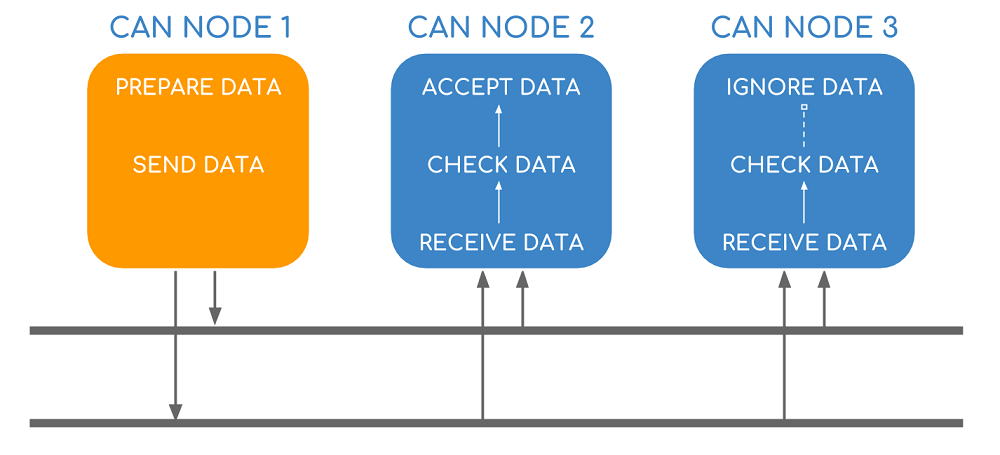
\includegraphics[scale=0.6]{images/principeCAN.png}
		\caption{Principe CAN}
	\end{center}
\end{figure}

\subsection{Comparaison}

\section{Sans-fil}

\subsection{TCP/IP}

\part{Automatique}

Le livre "Probabilistic Robotics" est excellent pour découvrir les différents problèmes de robotique. Il sert de très bonne introduction aux algorithmes de fusion de données pour estimer la position, au contrôle de robots et au SLAM.

\part{Machine learning}
On ne verra ici que les cas qui peuvent être utile pour la robotique.

\chapter{Apprentissage supervisé}

\section{Reconnaissance d'images}

\chapter{Reinforcement learning}

\section{Loi de commande de robot}

\part{Outils de la menuiserie}

\chapter{Les machines}
La menuiserie possède pas mal d'équipement à la disposition des élèves. Il n'y a pas trop de restrictions sur leur utilisation à condition de tout ranger après à moins de vouloir faire face à Jacky, le responsable de la menuiserie. Il ne faut d'ailleurs pas hésiter à lui demander conseil si besoin est, il est toujours prêt à aider les étudiants dans leurs projets.

Le responsable des outils avancés de la menuiserie est Henri Proudhon. C'est celui qu'il faut contacter si jamais vous souhaitez apprendre à utiliser l'une des machines.

\section{L'imprimante 3D}
L'école possède pour l'instant 3 imprimantes 3D. Vous n'utiliserez très probablement jamais la plus ancienne. Les 2 que seront utiles sont:
\begin{description}
\item[l'Ultimaker 2+:]C'est celle qui peut imprimer le plus grand volume: 223 x 223 x 305 mm
\item[l'Ultimaker 3:]La version la plus récente. Elle permet d'imprimer un volume plus faible que l'Ultimaker 2+ (215 x 215 x 200 mm) mais elle possède 2 têtes d'impressions ce qui lui permet de faire des impressions avec 2 matériaux différents.
\end{description}

\begin{figure}[h!]
	\begin{center}
		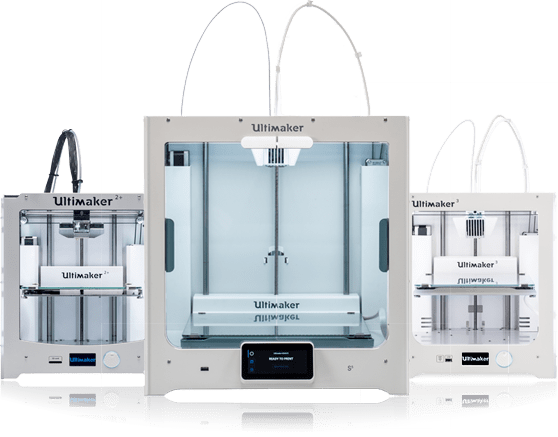
\includegraphics[scale=0.6]{images/ultimaker.png}
		\caption{Les imprimantes 3D Ultimaker}
	\end{center}
\end{figure}

\subsection{Le logiciel: Cura}
Cura est le logiciel qui permet de créer le fichier qui sera utilisé par les Ultimakers. On peut définir les paramètres d'impressions et le positionnement des objets à imprimer dans l'imprimante 3D. 

Attention, l'Ultimaker 3 ne fonctionne pas pour l'instant avec la version 3.3.1 de Cura. Il faut utiliser la version 3.2.1.

\begin{figure}[h!]
	\begin{center}
		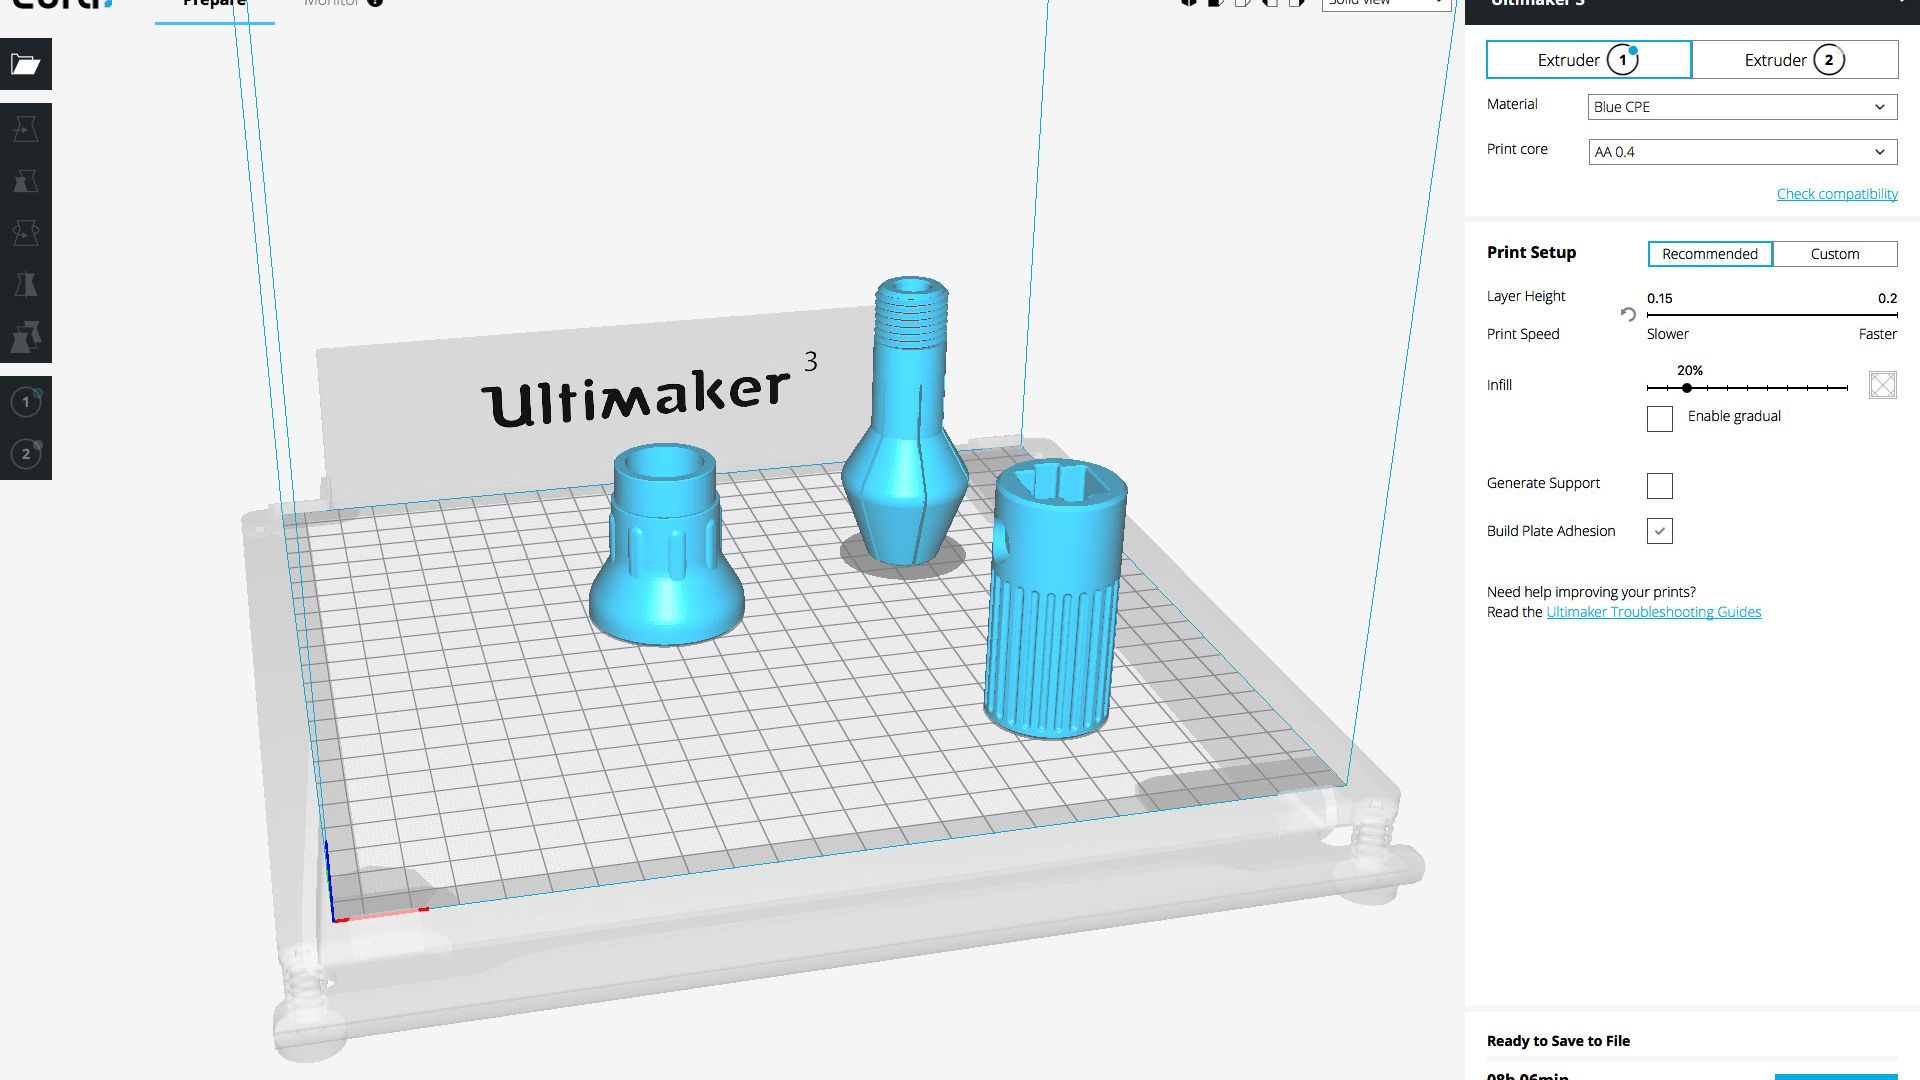
\includegraphics[width=0.5\textwidth]{images/cura.jpg}
		\caption{Cura}
	\end{center}
\end{figure}

\subsection{Utilisation}
Avant de lancer l'impression, il faut passer un coup de spray dur le plateau d'impression. Cela évite d'avoir des problèmes quand on décollera l'impression à la fin.

Le menu est très intuitif et bien expliqué. Le changement des bobines est aussi très simple et bien expliqué sur le site web d'Ultimaker.

\section{La découpeuse laser}
La découpeuse laser est plus complexe à utiliser que l'imprimante 3D. Il vaut mieux que Henri Proudhon vous montre précisément comment l'utiliser. Il faut en effet choisir des paramètres spécifiques à chaque matériaux. Des paramètres sont déjà définis dans la machine pour certains matériaux mais il faudra très certainement mettre cela à jour avec de nouveaux matières premières. Ensuite, il faut calibrer la distance du laser au matériau à découper afin que cela corresponde à la distance focale. C'est d'ailleurs pour cela qu'il est impossible de couper des matériaux d'une trop grande épaisseur (21mm ne passent pas je crois). On peut contourner ce problème en découpant plusieurs fois le même motif et en les empilant par contre.

La découpeuse laser accepte seulement des matériaux de 40 x 80 cm (à revérifier). Cependant, la découpeuse laser s'ouvre sur un côté. Cela permet d'insérer dedans de pièces qui font plus de 40 cm de largeur.

Certaines matières plastiques ne peuvent être découpées par la découpeuse laser car ils produisent des fumées toxiques lorsqu'ils brûlent. Il faut alors utiliser une fraiseuse CNC (qui est en réparation).

\begin{figure}[h!]
	\begin{center}
		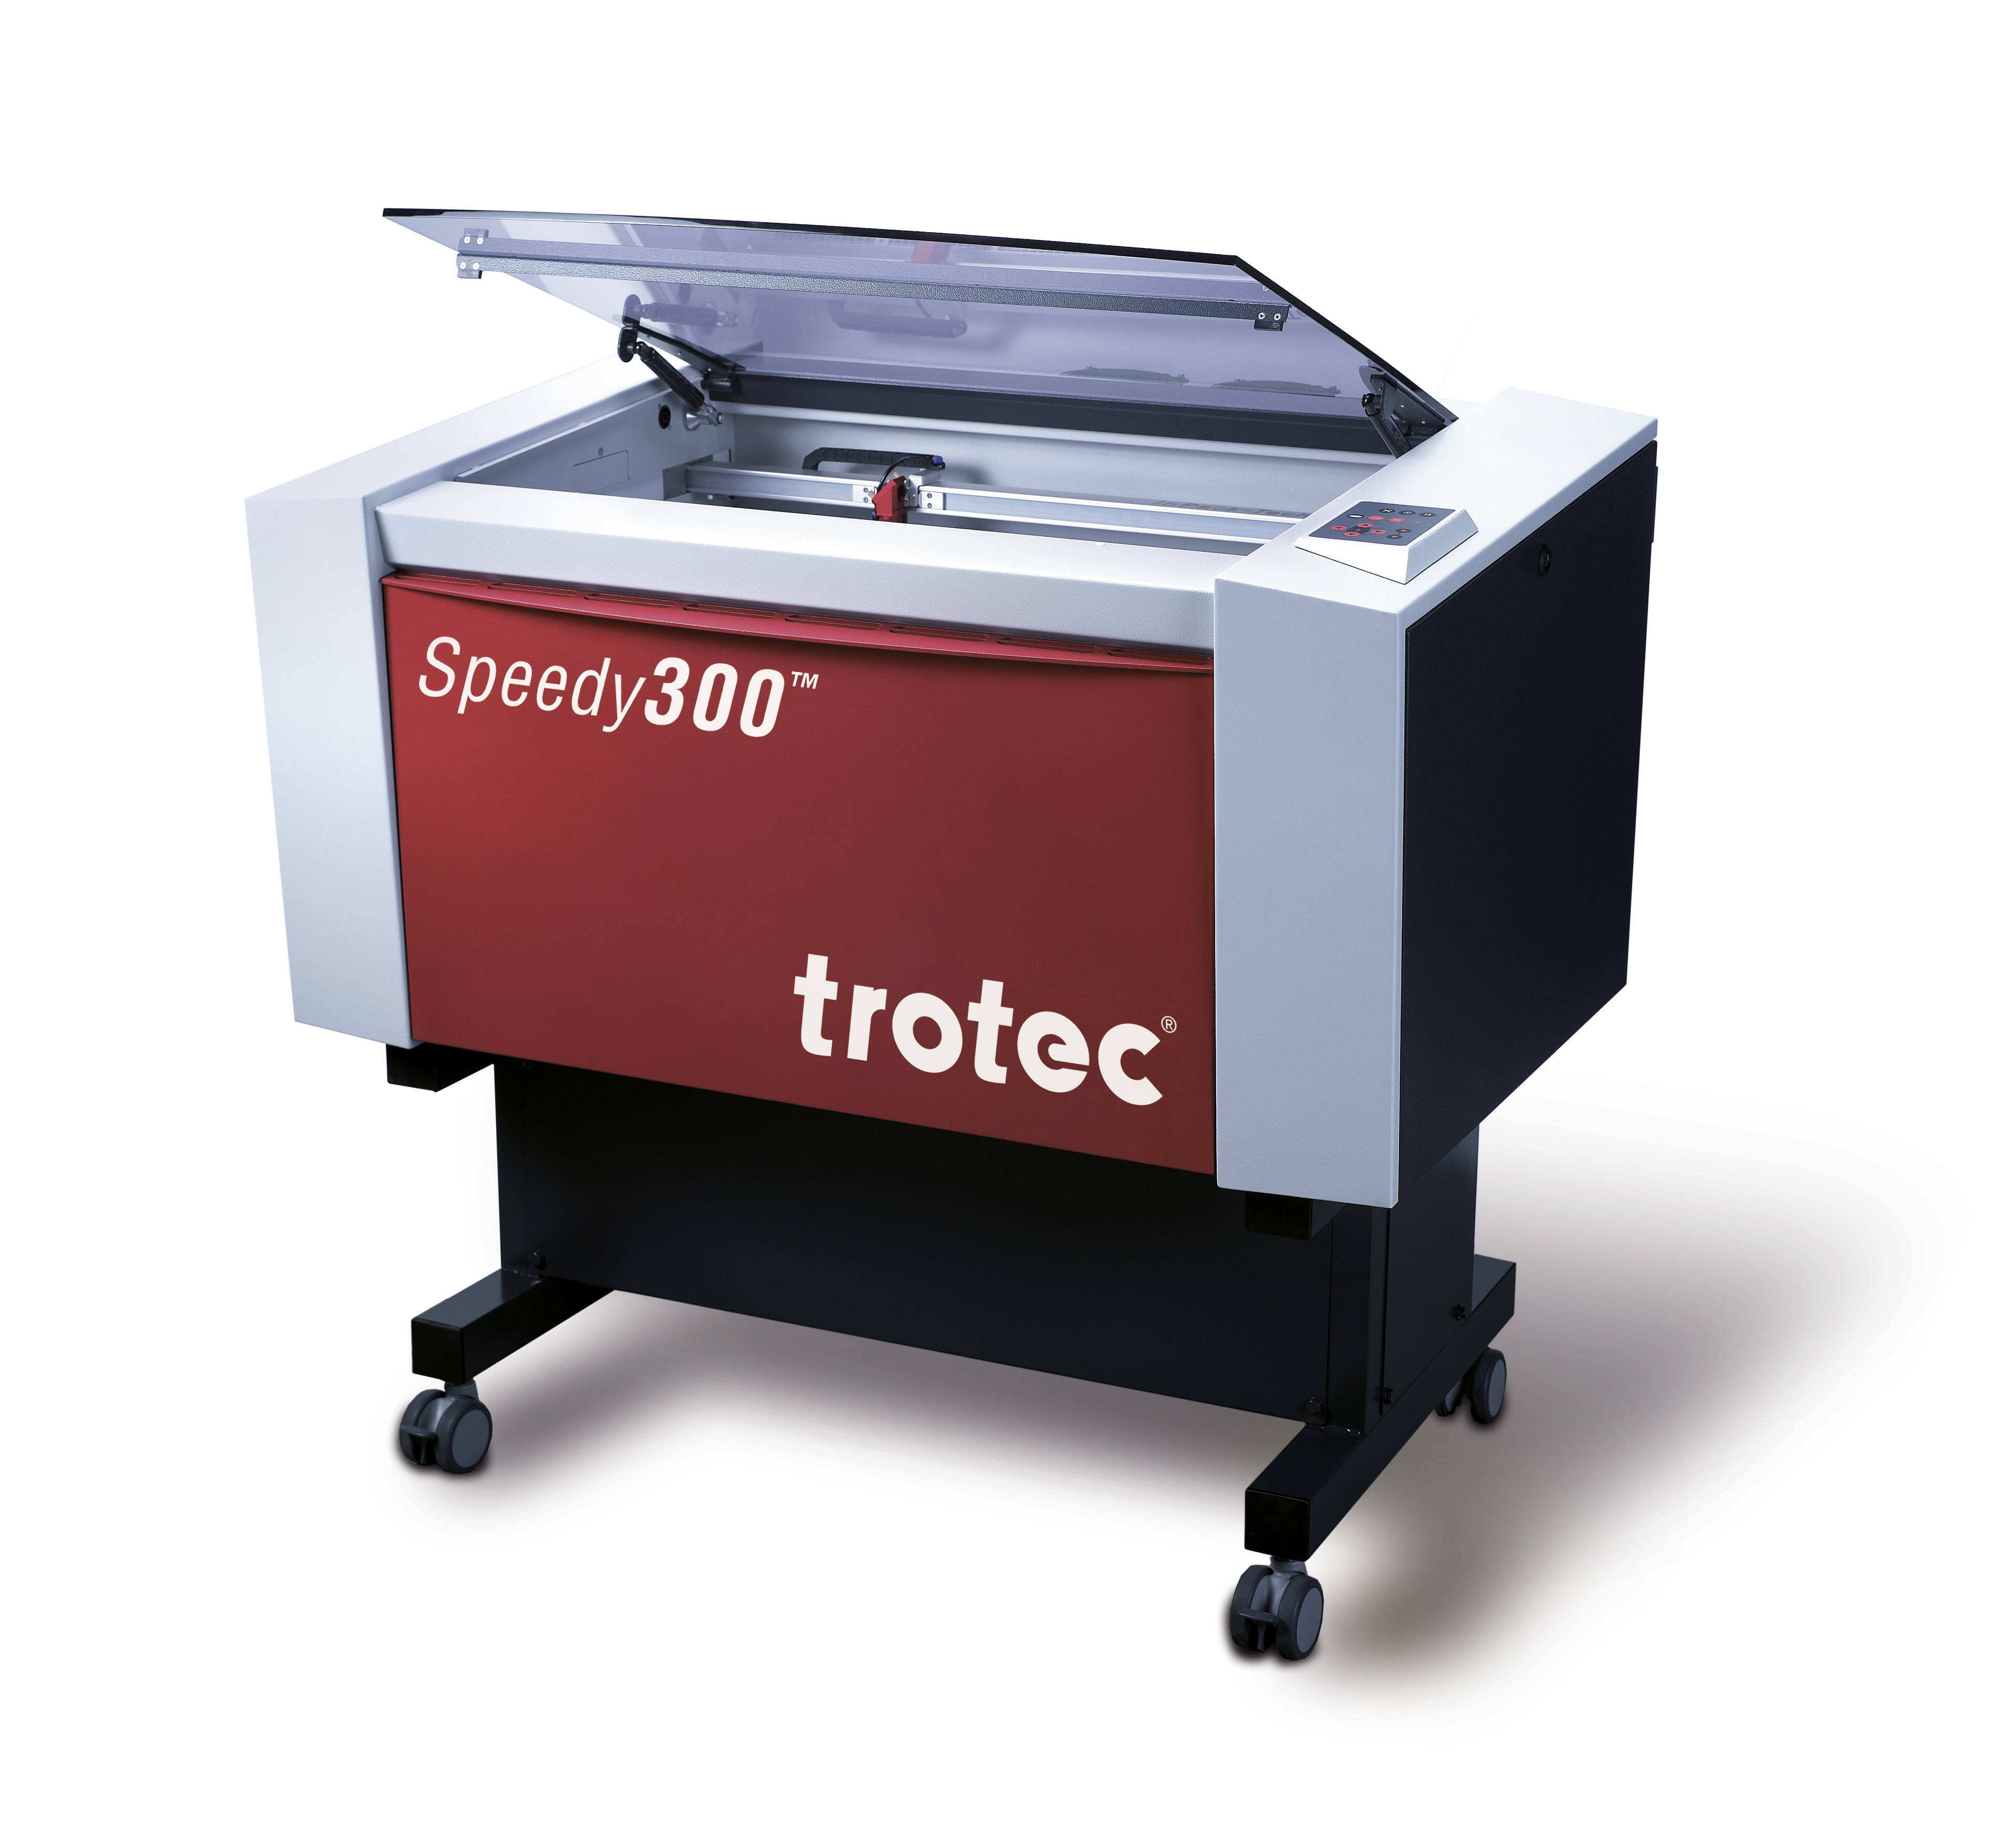
\includegraphics[width=0.5\textwidth]{images/decoupeuse_laser.jpg}
		\caption{Découpeuse laser}
	\end{center}
\end{figure}

\subsection{Le logiciel: Inkscape}
Inkscape est un logiciel de traitement graphique. C'est celui qui produit les fichiers acceptés par la découpeuse laser. Si vous souhaitez découper quelque chose, il faut que votre dessin soit importer sous Inkscape, mis à l'échelle (attention aux unités utilisés) puis il faut que le trait soit en rouge afin qu'il soit reconnu par la découpeuse laser.

\begin{figure}[h!]
	\begin{center}
		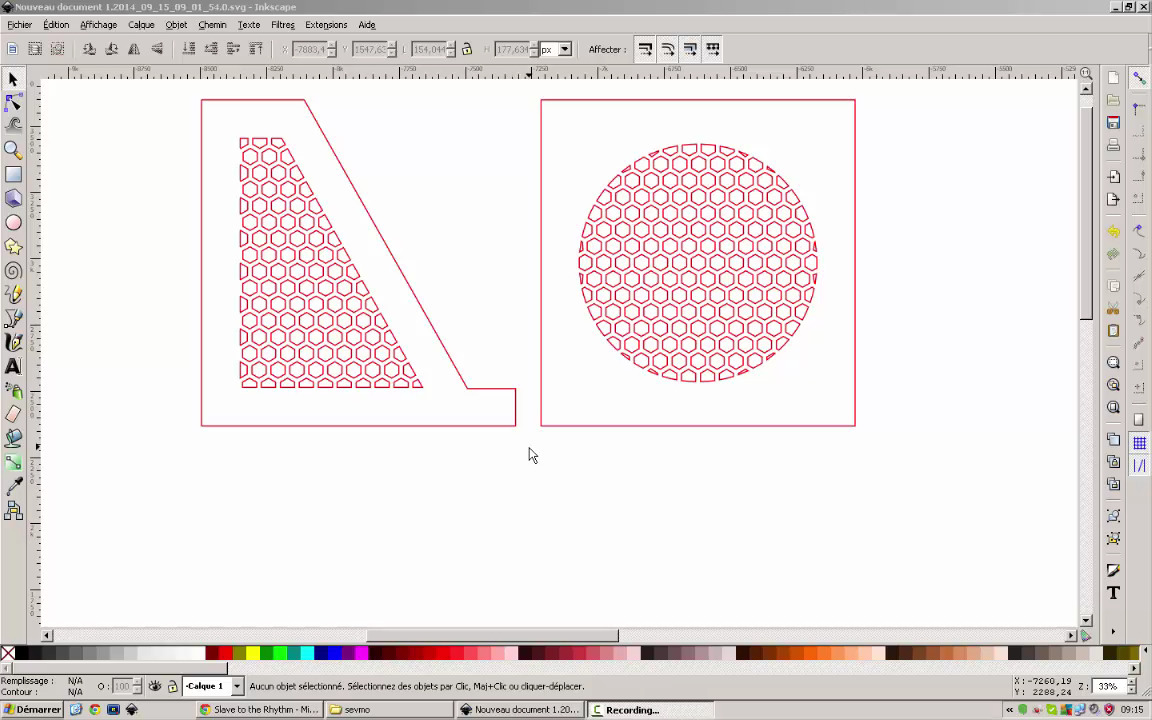
\includegraphics[width=0.5\textwidth]{images/inkscape.jpg}
		\caption{Inkscape}
	\end{center}
\end{figure}

\part{Conception}

\chapter{Général}

La règle d'or doit toujours être la SIMPLICITÉ. Il faut un système robuste et très répétable. Il y a toujours des imprévus (dimension de la table ou des objets à manipuler notamment).

\chapter{CAO}

\part{La Coupe de France de Robotique}

\chapter{Pendant l'année}
\begin{itemize}
\item Dès que du matériel est nécessaire, le commander immédiatement afin de l’avoir pour la semaine d’après. C’est souvent le matériel qui empêche de progresser sur les robots et de faire des test.
\item Garder l'un des robots de la compétition précédente afin de pouvoir avoir dès le début une base roulante. Cela permettra de commencer directement à coder et à faire des tests pour des algo de pathfinding ou d'évitement d'obstacles.
\end{itemize}
\chapter{Le départ}
\begin{itemize}
\item Une personne doit être responsable de l'intégralité du chargement des voitures afin d'être certain de ne rien oublier. Si plusieurs personnes s'en occupe et que la communication est mauvaise, il y aura des oublis (oublier les vis de la table de jeu par exemple)
\item Faire une liste des outils et matières premières une semaine à l’avance afin de ne rien oublier. Il faudra cette liste à Mazouz.
\item Trouver un moyen pour déplacer les 2 robots et l’équipement nécessaire pour les préparer avec une seule personne. En effet, seulement 2 personnes peuvent aller jusqu’à la table de match et il peut être dur de tout porter à 2. Cela peut être un petit chariot comme le font d’autres équipes.
\end{itemize}

\chapter{La compétition}

\section{Les matchs}
\begin{itemize}
\item Faire une checklist de toutes les tâches à effectuer pour préparer le match. Avec le stress, il n’est pas rare d’oublier quelque chose et de faire rater le match.
\item Éviter vraiment de faire des changements de dernière minute. En 2017, RCV a perdu en demi-finale car ils ont choisi une stratégie non-testée. Un bug a empêché les 2 robots de démarrer.
\end{itemize}

\part{Autres}

\chapter{Ressources utiles}

Site web:
\begin{description}
\item[Aéromodélisme et drone:] oscarliang.com
\end{description}

\end{document}
